\documentclass[journal,10pt,onecolumn]{IEEEtran}
\usepackage{graphicx}
\usepackage[margin=0.5in]{geometry}
\usepackage[cmex10]{amsmath}
\usepackage{amssymb}
\usepackage{array}
\usepackage{booktabs}
\usepackage{mathtools}
\usepackage{dirtree}
\usepackage{xcolor}
\usepackage{float}
\usepackage[justification=centering,font={rm,md,scriptsize}]{caption}
\usepackage{enumitem}
\usepackage{listings}
\usepackage{mathtools}
\usepackage{fancyvrb}
%\usepackage{hyperref}


%Add chapter functionality in IEEEtran class
\newcounter{Chapcounter}
\newcommand\showmycounter{\addtocounter{Chapcounter}{1}\themycounter}
\newcommand{\chapter}[1] 
{ {\centering          
  \addtocounter{Chapcounter}{1} \large \textbf{Chapter \theChapcounter ~#1}}  
  \addcontentsline{toc}{section}{Chapter ~\theChapcounter~~ #1}    
  \setcounter{section}{0}
}
%%%%

\counterwithin{enumi}{section}
\counterwithin{equation}{enumi}
\counterwithin{figure}{enumi}

\renewcommand\thesection{\theChapcounter.\arabic{section}}
\renewcommand\thesectiondis{\theChapcounter.\arabic{section}}
\newcommand\figref{Fig.~\ref}

\setenumerate{label=\thesection.\arabic*}

\lstset{
  basicstyle=\ttfamily,
  columns=fullflexible,
  frame=single,
  breaklines=true,
  postbreak=\mbox{\textcolor{red}{$\hookrightarrow$}\space},
}

\providecommand{\mbf}{\mathbf}
\providecommand{\pr}[1]{\ensuremath{\Pr\left(#1\right)}}
\providecommand{\qfunc}[1]{\ensuremath{Q\left(#1\right)}}
\providecommand{\sbrak}[1]{\ensuremath{{}\left[#1\right]}}
\providecommand{\lsbrak}[1]{\ensuremath{{}\left[#1\right.}}
\providecommand{\rsbrak}[1]{\ensuremath{{}\left.#1\right]}}
\providecommand{\brak}[1]{\ensuremath{\left(#1\right)}}
\providecommand{\lbrak}[1]{\ensuremath{\left(#1\right.}}
\providecommand{\rbrak}[1]{\ensuremath{\left.#1\right)}}
\providecommand{\cbrak}[1]{\ensuremath{\left\{#1\right\}}}
\providecommand{\lcbrak}[1]{\ensuremath{\left\{#1\right.}}
\providecommand{\rcbrak}[1]{\ensuremath{\left.#1\right\}}}
\newcommand{\sgn}{\mathop{\mathrm{sgn}}}
\providecommand{\abs}[1]{\left\vert#1\right\vert}
\providecommand{\res}[1]{\Res\displaylimits_{#1}} 
\providecommand{\norm}[1]{\left\lVert#1\right\rVert}
\providecommand{\mtx}[1]{\mathbf{#1}}
\providecommand{\mean}[1]{E\left[ #1 \right]}
\providecommand{\fourier}{\overset{\mathcal{F}}{ \rightleftharpoons}}
\providecommand{\ztrans}{\overset{\mathcal{Z}}{ \rightleftharpoons}}
\providecommand{\system}{\overset{\mathcal{H}}{ \longleftrightarrow}}
\newcommand{\solution}{\noindent \textbf{Solution: }}
\newcommand{\cosec}{\,\text{cosec}\,}
\providecommand{\dec}[2]{\ensuremath{\overset{#1}{\underset{#2}{\gtrless}}}}
\newcommand{\myvec}[1]{\ensuremath{\begin{pmatrix}#1\end{pmatrix}}}
\newcommand{\mydet}[1]{\ensuremath{\begin{vmatrix}#1\end{vmatrix}}}
\providecommand{\gauss}[2]{\mathcal{N}\ensuremath{\left(#1,#2\right)}}
\newcommand*{\permcomb}[4][0mu]{{{}^{#3}\mkern#1#2_{#4}}}
\newcommand*{\perm}[1][-3mu]{\permcomb[#1]{P}}
\newcommand*{\comb}[1][-1mu]{\permcomb[#1]{C}}

\let\vec\mathbf

\def\putbox#1#2#3{\makebox[0in][l]{\makebox[#1][l]{}\raisebox{\baselineskip}[0in][0in]{\raisebox{#2}[0in][0in]{#3}}}}
     \def\rightbox#1{\makebox[0in][r]{#1}}
     \def\centbox#1{\makebox[0in]{#1}}
     \def\topbox#1{\raisebox{-\baselineskip}[0in][0in]{#1}}
     \def\midbox#1{\raisebox{-0.5\baselineskip}[0in][0in]{#1}}

\begin{document}

\title{\textbf{Digital Communication}}
\author{M. Dinesh-(FWC22044)}
\date{January 2023}

\maketitle

\tableofcontents

\bigskip
\chapter{Two Dice}









\section{Sum of Independant Random Variables}



Two dice, one blue and one grey, are thrown at the same time.   The event defined by the sum of the two numbers appearing on the top of the dice can have 11 possible outcomes 2, 3, 4, 5, 6, 6, 8, 9, 10, 11 and 12.  A student argues that each of these outcomes has a probability $\frac{1}{11}$.  Do you agree with this argument?  Justify your answer.





\begin{enumerate}
\item  {\em The Uniform Distribution: }Let $X_i \in \cbrak{1,2,3,4,5,6}, i = 1,2,$ be the random variables representing the outcome for each die.  Assuming the dice to be fair, the probability mass function pmf) is expressed as 
\begin{align}
\label{eq:dice_pmf_xi}
p_{X_i}(n) = \pr{X_i = n} = 
\begin{cases}
\frac{1}{6} & 1 \le n \le 6
\\
0 & otherwise
\end{cases}
\end{align}
The desired outcome is
\begin{align}
\label{eq:dice_xdef}
X &= X_1 + X_2,
\\
\implies X &\in \cbrak{1,2,\dots,12}
\end{align}
%
The objective is to show that
\begin{align}
p_X(n) \ne \frac{1}{11}
\label{eq:dice_wrong}
\end{align}
\item {\em Convolution: }
From \eqref{eq:dice_xdef},
\begin{align}
p_X(n) &= \pr{X_1 + X_2 = n} = \pr{X_1  = n -X_2}
\\
&= \sum_{k}^{}\pr{X_1  = n -k | X_2 = k}p_{X_2}(k)
\label{eq:dice_x_sum}
\end{align}%
after unconditioning.  $\because X_1$ and $X_2$ are independent,
\begin{multline}
\pr{X_1  = n -k | X_2 = k} 
\\
= \pr{X_1  = n -k} = p_{X_1}(n-k)
\label{eq:dice_x1_indep}
\end{multline}
From \eqref{eq:dice_x_sum} and \eqref{eq:dice_x1_indep},
\begin{align}
p_X(n) = \sum_{k}^{}p_{X_1}(n-k)p_{X_2}(k) = p_{X_1}(n)*p_{X_2}(n)
\label{eq:dice_x_conv}
\end{align}
where $*$ denotes the convolution operation. 
%\cite{proakis_dsp}.  
Substituting from \eqref{eq:dice_pmf_xi}
in \eqref{eq:dice_x_conv},
\begin{align}
p_X(n) = \frac{1}{6}\sum_{k=1}^{6}p_{X_1}(n-k)= \frac{1}{6}\sum_{k=n-6}^{n-1}p_{X_1}(k)
\label{eq:dice_x_conv_x1}
\end{align}
\begin{align}
\because p_{X_1}(k) &= 0, \quad k \le 1, k \ge 6.
\end{align}
From \eqref{eq:dice_x_conv_x1},
%
\begin{align}
p_X(n) &= 
\begin{cases}
0 & n < 1
\\
\frac{1}{6}\sum_{k=1}^{n-1}p_{X_1}(k) &  1 \le n-1 \le  6
\\
\frac{1}{6}\sum_{k=n-6}^{6}p_{X_1}(k) & 1 < n-6 \le 6
\\
0 & n > 12
\end{cases}
\label{eq:dice_x_conv_cond}
\end{align}
Substituting from \eqref{eq:dice_pmf_xi} in \eqref{eq:dice_x_conv_cond},
\begin{align}
p_X(n) &= 
\begin{cases}
0 & n < 1
\\
\frac{n-1}{36} &  2 \le n \le  7
\\
\frac{13-n}{36} & 7 < n \le 12
\\
0 & n > 12
\end{cases}
\label{eq:dice_x_conv_final}
\end{align}
satisfying \eqref{eq:dice_wrong}.
\item {\em The $Z$-transform: }
The $Z$-transform of $p_X(n)$ is defined as 
%\cite{proakis_dsp}
\begin{align}
P_X(z) = \sum_{n = -\infty}^{\infty}p_X(n)z^{-n}, \quad z \in \mathbb{C}
\label{eq:dice_xz}
\end{align}
%
From \eqref{eq:dice_pmf_xi} and \eqref{eq:dice_xz}, 
\begin{align}
P_{X_1}(z) =P_{X_2}(z) &= \frac{1}{6}\sum_{n = 1}^{6}z^{-n}
\\
&=\frac{z^{-1}\brak{1-z^{-6}}}{6\brak{1-z^{-1}}}, \quad \abs{z} > 1
\label{eq:dice_xiz}
\end{align}
upon summing up the geometric progression.  
\begin{align}
\because p_X(n) &= p_{X_1}(n)*p_{X_2}(n),
\\
P_X(z) &= P_{X_1}(z)P_{X_2}(z)
\label{eq:dice_xzprod_def}
\end{align}
The above property follows from Fourier analysis and is fundamental to signal processing. 
%\cite{proakis_dsp}. 
From \eqref{eq:dice_xiz} and \eqref{eq:dice_xzprod_def},
\begin{align}
P_X(z) &= \cbrak{\frac{z^{-1}\brak{1-z^{-6}}}{6\brak{1-z^{-1}}}}^2
\\
&= \frac{1}{36}\frac{z^{-2}\brak{1-2z^{-6}+z^{-12}}}{\brak{1-z^{-1}}^2}
\label{eq:dice_xzprod}
\end{align}
Using the fact that 
%\cite{proakis_dsp}
\begin{align}
p_X(n-k) &\system{Z}P_X(z)z^{-k},
\\
nu(n)&\system{Z} \frac{z^{-1}}{\brak{1-z^{-1}}^2}
\end{align}
after some algebra, it can be shown that
%{\tiny
\begin{multline}
\frac{1}{36}\lsbrak{\brak{n-1}u(n-1) - 2 \brak{n-7}u(n-7)}
\\
\rsbrak{ +\brak{n-13}u(n-13)}
\\
\system{Z}
\frac{1}{36}\frac{z^{-2}\brak{1-2z^{-6}+z^{-12}}}{\brak{1-z^{-1}}^2}
\label{eq:dice_xz_closed}
\end{multline}
%}

where 
\begin{align}
u(n) =
\begin{cases}
1 & n \ge 0
\\
0 & n < 0
\end{cases}
\end{align}

From \eqref{eq:dice_xz}, \eqref{eq:dice_xzprod} and \eqref{eq:dice_xz_closed}
\begin{multline}
p_{X}(n) = \frac{1}{36}\lsbrak{\brak{n-1}u(n-1) 
}
\\
\rsbrak{- 2 \brak{n-7}u(n-7)+\brak{n-13}u(n-13)}
\end{multline}
which is the same as \eqref{eq:dice_x_conv_final}.  Note that  \eqref{eq:dice_x_conv_final} can be obtained from \eqref{eq:dice_xz_closed} using contour integration as well.
% \cite{proakis_dsp}.  

\item 
The experiment of rolling the dice was simulated using Python for 10000 samples.  These were generated using Python libraries for uniform distribution. The frequencies for each outcome were then used to compute the resulting pmf, which  is plotted in Figure \ref{fig:dice}.  The theoretical pmf obtained in \eqref{eq:dice_x_conv_final} is plotted for comparison.  
%
\begin{figure}[H]
\centering
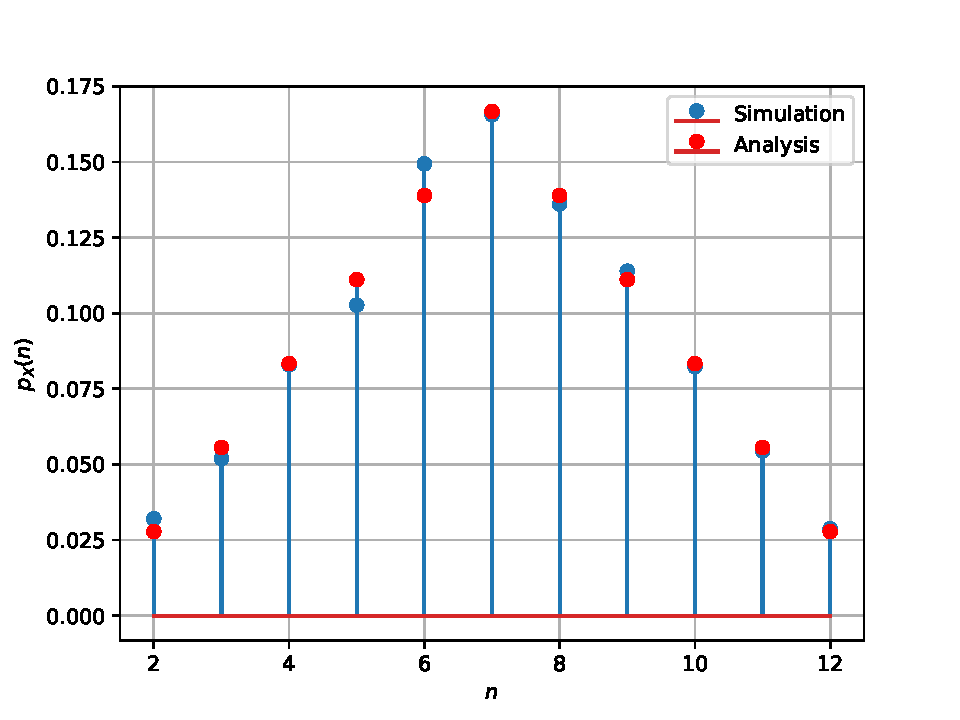
\includegraphics[width=\columnwidth]{./figs/chapter1/pmf.pdf}
\caption{Plot of $p_X(n)$.  Simulations are close to the analysis. }
\label{fig:dice}
\end{figure}
\item The python code is available in 
\begin{lstlisting}
/codes/ch1/dice.py
\end{lstlisting}

\end{enumerate}

\chapter{Random Numbers}
\section{Uniform Random Numbers}
Let $U$ be a uniform random variable between 0 and 1.
\begin{enumerate}
\item Generate $10^6$ samples of $U$ using a C program and save into a file called uni.dat .
\label{prob:uni_gen}
\\
\solution Download the following files and execute the  C program.
\begin{lstlisting}
codes/include/coeffs.h
codes/ch2/uni.c
\end{lstlisting}

%
\item
Load the uni.dat file into python and plot the empirical CDF of $U$ using the samples in uni.dat. The CDF is defined as
\begin{align}
F_{U}(x) = \pr{U \le x}
\end{align}
\\
\solution  The following code plots \figref{fig:uni_cdf}
\begin{lstlisting}
codes/ch2/uni_cdf.py
\end{lstlisting}
\begin{figure}[H]
\centering
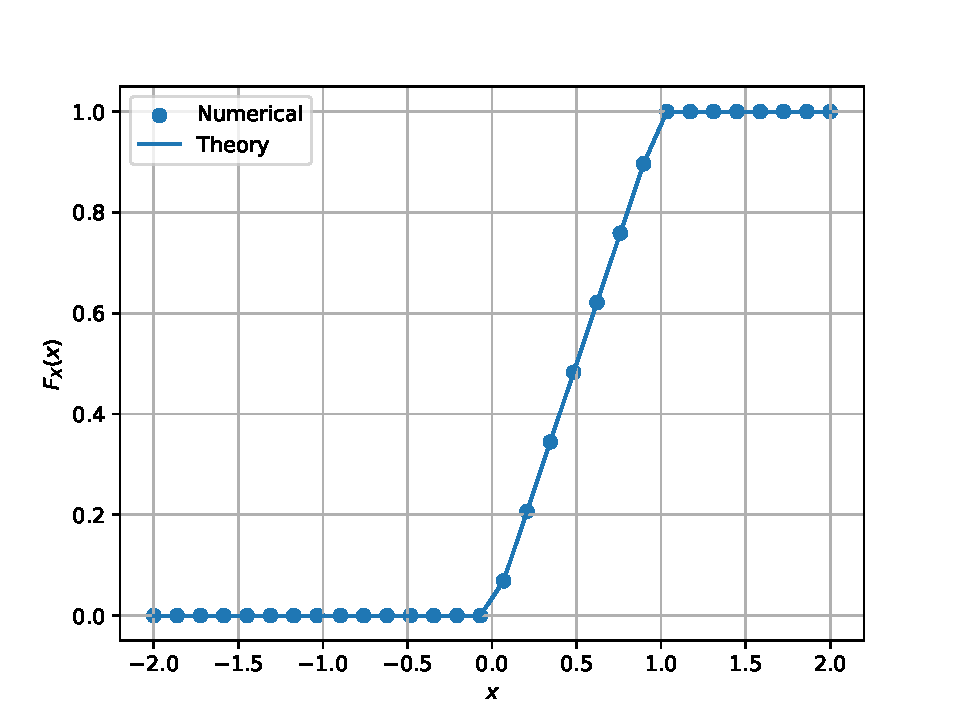
\includegraphics[width=\columnwidth]{./figs/chapter2/uni_cdf.pdf}
\caption{The CDF of $U$}
\label{fig:uni_cdf}
\end{figure}

%
\item
Find a  theoretical expression for $F_{U}(x)$.\\
\solution
\begin{align} 
F_{U}(x) = \int_{-\infty}^{x} f_{U}(x)\,dx
\label{eq:pdf_to_cdf}
\end{align}
For the uniform random variable $U$, $f_{U}(x)$ is given by  
\begin{align}
	f_U(x) &= 
	\begin{cases}
	1 &  0 \le x \le  1
	\\
	0 & elsewhere
	\\
	\end{cases}
	\label{eq:uni_pdf}
\end{align}
Substituting \eqref{eq:uni_pdf} in \eqref{eq:pdf_to_cdf}, $F_U(x)$ is found to be
\begin{align}
	F_U(x) &= 
	\begin{cases}
	0 & x < 0
	\\	
	x & 0 \le x \le  1
	\\
	1 & x > 0
	\\
	\end{cases}
	\label{eq:uni_cdf}
\end{align}

\item
\label{prob:print_uni}
The mean of $U$ is defined as
%
\begin{equation}
E\sbrak{U} = \frac{1}{N}\sum_{i=1}^{N}U_i
\end{equation}
%
and its variance as
%
\begin{equation}
\text{var}\sbrak{U} = E\sbrak{U- E\sbrak{U}}^2 
\end{equation}

Write a C program to  find the mean and variance of $U$.\\
\solution The following code prints the mean and variance of $U$
\begin{lstlisting}
codes/ch2/uni.c
\end{lstlisting}
The output of the program is
\begin{lstlisting}
Uniform stats:
Mean: 0.500007
Variance: 0.083301
\end{lstlisting}

\item Verify your result theoretically given that
%
\begin{equation}
E\sbrak{U^k} = \int_{-\infty}^{\infty}x^kdF_{U}(x)
\end{equation}\\
\solution For a random variable $X$, the mean $\mu_X$ and variance $\sigma_X^2$ are given by
\begin{align}
	\label{eq:mean_exp}
	\mu_X &= E\sbrak{X} = \int_{-\infty}^{\infty}xdF_{U}(x) \\
	\label{eq:var_exp}
	\sigma_X^2 &= E\sbrak{X^2} - \mu_X^2 = \int_{-\infty}^{\infty}x^2dF_{U}(x) - \mu_X^2
\end{align}  
Substituting the CDF of $U$ from \eqref{eq:uni_cdf} in \eqref{eq:mean_exp} and \eqref{eq:var_exp}, we get
\begin{align}
	\label{eq:mean_uni}
	\mu_U &= \frac{1}{2} \\
	\label{eq:var_uni}
	\sigma_U^2 &= \frac{1}{12}
\end{align}  
which match with the values printed in problem \ref{prob:print_uni}
\end{enumerate}
\section{Central Limit Theorem}
\begin{enumerate}
%
%
\item
Generate $10^6$ samples of the random variable
%
\begin{equation}
X = \sum_{i=1}^{12}U_i -6
\end{equation}
%
using a C program, where $U_i, i = 1,2,\dots, 12$ are  a set of independent uniform random variables between 0 and 1
and save in a file called gau.dat\\
\solution Download the following files and execute the  C program.
\begin{lstlisting}
codes/include/coeffs.h
codes/ch2/gau.c
\end{lstlisting}
%
\item
Load gau.dat in python and plot the empirical CDF of $X$ using the samples in gau.dat. What properties does a CDF have?
\\
\solution The CDF of $X$ is plotted in \figref{fig:gauss_cdf}
\begin{figure}[H]
\centering
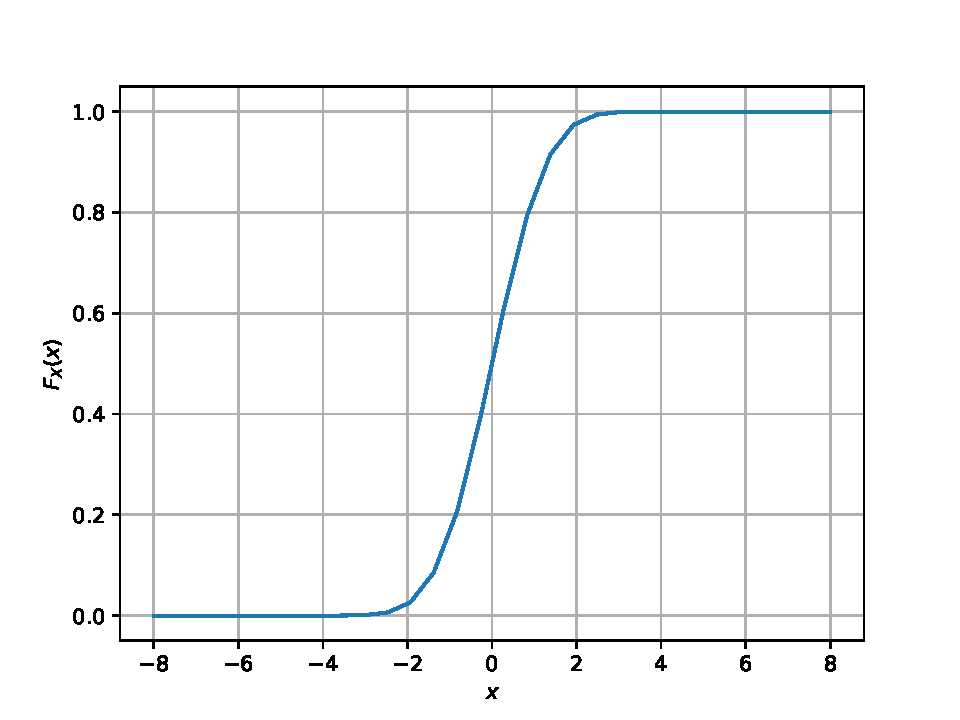
\includegraphics[width=\columnwidth]{./figs/chapter2/gau_cdf.pdf}
\caption{The CDF of $X$}
\label{fig:gauss_cdf}
\end{figure}
The properties of a CDF are
\begin{eqnarray}
	F_X(-\infty) = 0\\
	F_X(\infty) = 1\\
	\frac{dF_X(x)}{dx} \ge 0
\end{eqnarray}
\item
Load gau.dat in python and plot the empirical PDF of $X$ using the samples in gau.dat. The PDF of $X$ is defined as
\begin{align}
p_{X}(x) = \frac{d}{dx}F_{X}(x)
\label{eq:cdf_to_pdf}
\end{align}
What properties does the PDF have?
\\
\solution The PDF of $X$ is plotted in \figref{fig:gauss_pdf} using the code below
\begin{lstlisting}
codes/ch2/gua_cdf_pdf_plot.py
\end{lstlisting}

\begin{figure}[H]
\centering
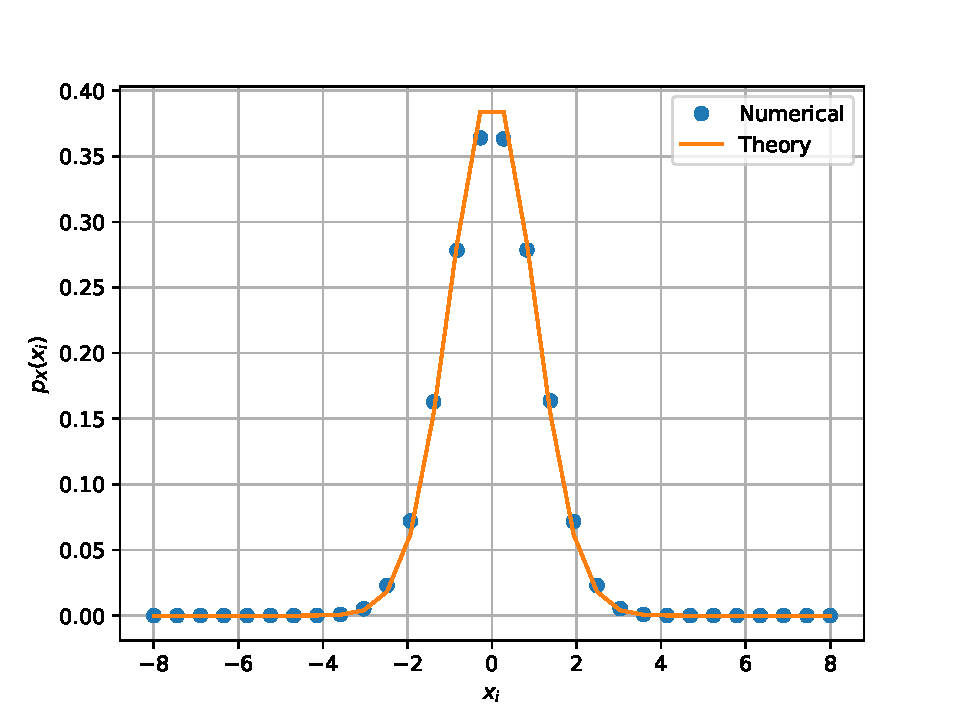
\includegraphics[width=\columnwidth]{./figs/chapter2/gau_pdf.pdf}
\caption{The PDF of $X$}
\label{fig:gauss_pdf}
\end{figure}

The properties of PDF are
\begin{eqnarray}
	f_X(x) \ge 0\\
	\int_{-\infty}^{\infty} f_X(x) \,dx = 1
\end{eqnarray}

\item Find the mean and variance of $X$ by writing a C program.
\solution The following code prints the mean and variance of $X$
\begin{lstlisting}
codes/ch2/gau.c
\end{lstlisting}
The output of the program is
\begin{lstlisting}
Gaussian stats:
Mean: 0.000294
Variance: 0.999562	
\end{lstlisting}
\item Given that 
\begin{align}
p_{X}(x) = \frac{1}{\sqrt{2\pi}}\exp\brak{-\frac{x^2}{2}}, -\infty < x < \infty,
\label{eq:gau_pdf}
\end{align}
repeat the above exercise theoretically.\\
\solution Substituting the PDF from \eqref{eq:gau_pdf} in \eqref{eq:mean_exp},
\begin{flalign}
	\mu_X &= \int_{-\infty}^{\infty} \frac{x}{\sqrt{2\pi}}\exp\brak{-\frac{x^2}{2}} \,dx&\\
	\intertext{Using}&\\
	\int x \cdot \exp \left( -a x^2 \right) \mathrm{d}x &= -\frac{1}{2a} \cdot \exp \left( -a x^2 \right)&\\
	\mu_X &= \frac{1}{\sqrt{2\pi}}\left[-\exp\brak{-\frac{x^2}{2}}\right]_{-\infty}^{\infty}&\\  
	\mu_X &= 0
\end{flalign}
Substituting $\mu_X$ and the PDF in \eqref{eq:var_exp} to compute variance,
\begin{flalign}
	\sigma_X^2 &= \int_{-\infty}^{\infty} \frac{x^2}{\sqrt{2\pi}}\exp\brak{-\frac{x^2}{2}} \,dx&\\ \nonumber
	\intertext{Substituting} t &= \frac{x^2}{2},&\\	
	\sigma_X^2 &= \frac{2}{\sqrt{\pi}} \int_{0}^{\infty} t^{\frac{1}{2}}\exp\brak{-t} \,dt&\\	\nonumber
	&= \frac{2}{\sqrt{\pi}} \int_{0}^{\infty} t^{\frac{3}{2}-1}\exp\brak{-t} \,dt&\\
	\intertext{Using the gamma function} \Gamma(x) &= \int_{0}^{\infty} z^{x-1} \cdot e^{-z} \, \mathrm{d}z \,&\\
	\sigma_X^2 &= \frac{2}{\sqrt{\pi}}\Gamma(\frac{3}{2})&\\	\nonumber
	&= \frac{2}{\sqrt{\pi}}\frac{\sqrt{\pi}}{2}&\\	\nonumber
	&=1	
\end{flalign}
%
\end{enumerate}
\section{From Uniform to Other}
\begin{enumerate}
%
\item
Generate samples of 
%
\begin{equation}
V = -2\ln\brak{1-U}
\end{equation}
%
and plot its CDF. \\
\solution The samples for $U$ are loaded from uni.dat file generated in problem \ref{prob:print_uni}. The CDF of $V$ is plotted in \figref{fig:log_uni_cdf} using the code below, 
\begin{lstlisting}
codes/ch2/nat.py
\end{lstlisting}
\begin{figure}[H]
\centering
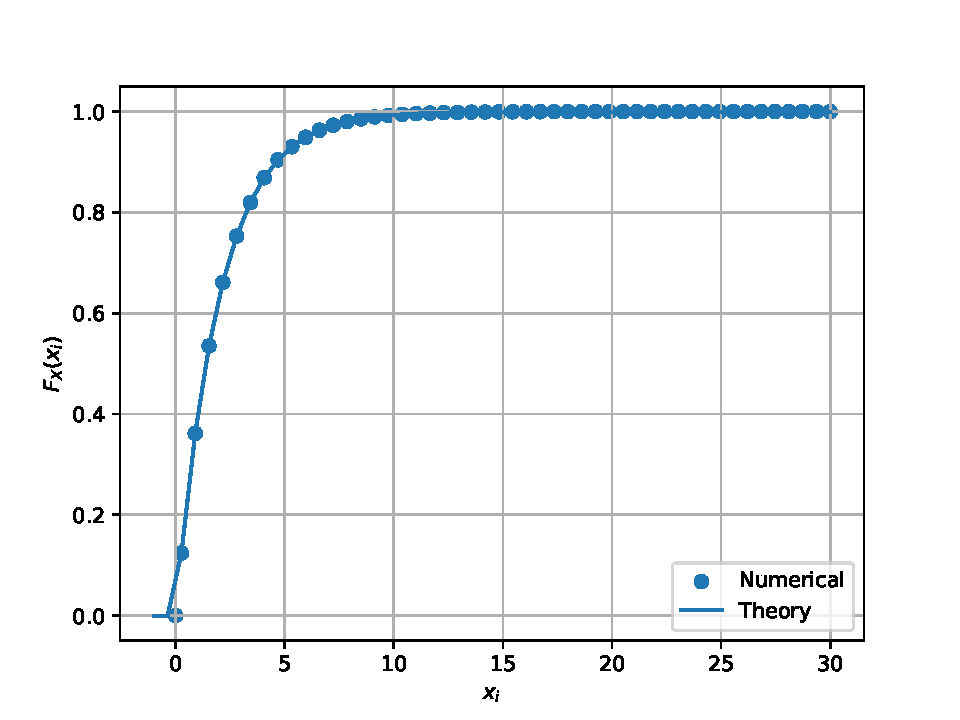
\includegraphics[width=\columnwidth]{./figs/chapter2/log_uni_cdf.pdf}
\caption{The CDF of $V$}
\label{fig:log_uni_cdf}
\end{figure}
\item Find a theoretical expression for $F_V(x)$.
\begin{flalign}
	F_V(x) &= P(V < x)&\\
	&= P(-2\ln\brak{1-U} < x)&\\
	&= P(U < 1 - e^{\frac{-x}{2}})&\\
	&= F_U(1 - e^{\frac{-x}{2}})
\end{flalign}
Using $F_U(x)$ defined in \eqref{eq:uni_cdf},
\begin{align}
	F_V(x) &=
	\begin{cases}
		0 & x < 0\\
		1 - e^{\frac{-x}{2}} & x \ge 0
	\end{cases}
\end{align} 
%
%\item
%Generate the Rayleigh distribution from Uniform. Verify your result through graphical plots.
\end{enumerate}

\section{Triangular Distribution}
%
\begin{enumerate}
\item Generate 
	\begin{align}
		T = U_1+U_2
	\end{align}\\
\solution Download the following files and execute the  C program.
\begin{lstlisting}
codes/include/coeffs.h
codes/ch2/two_uni.c
\end{lstlisting}
\item Find the CDF of $T$.\\
\solution Loading the samples from uni1.dat and uni2.dat in python, the CDF is plotted in \figref{fig:tri_cdf} 
\begin{figure}[H]
\centering
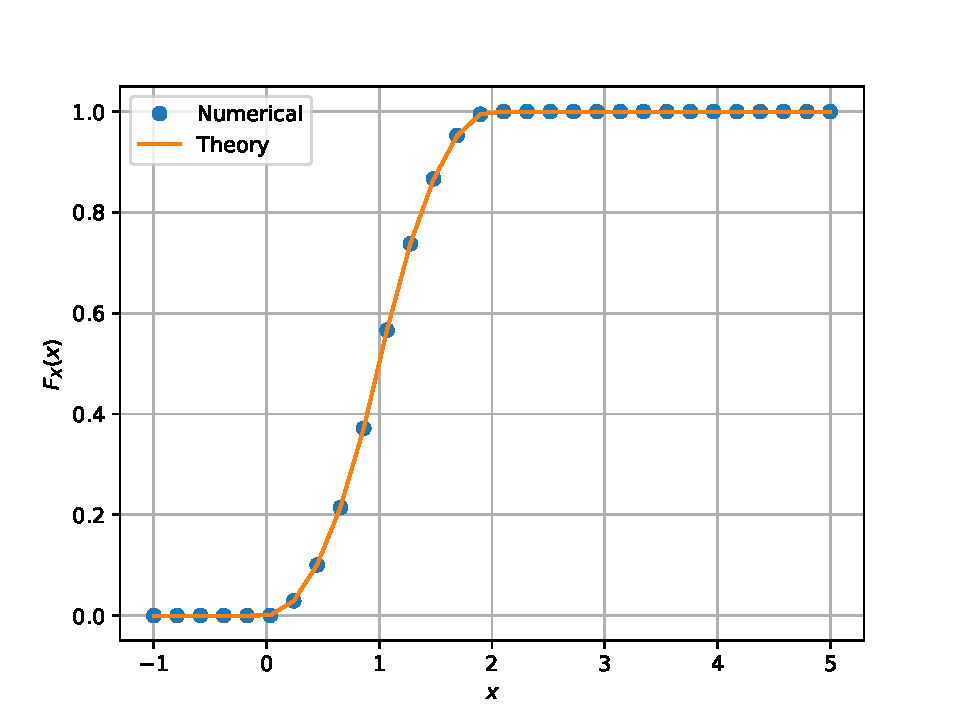
\includegraphics[width=\columnwidth]{./figs/chapter2/tri_cdf.pdf}
\caption{The CDF of $T$}
\label{fig:tri_cdf}
\end{figure}
\item Find the PDF of $T$.\\
\solution The PDF of $T$ is plotted in \figref{fig:tri_pdf} using the code below
\begin{lstlisting}
codes/ch2/tri.py
\end{lstlisting}
\begin{figure}[H]
\centering
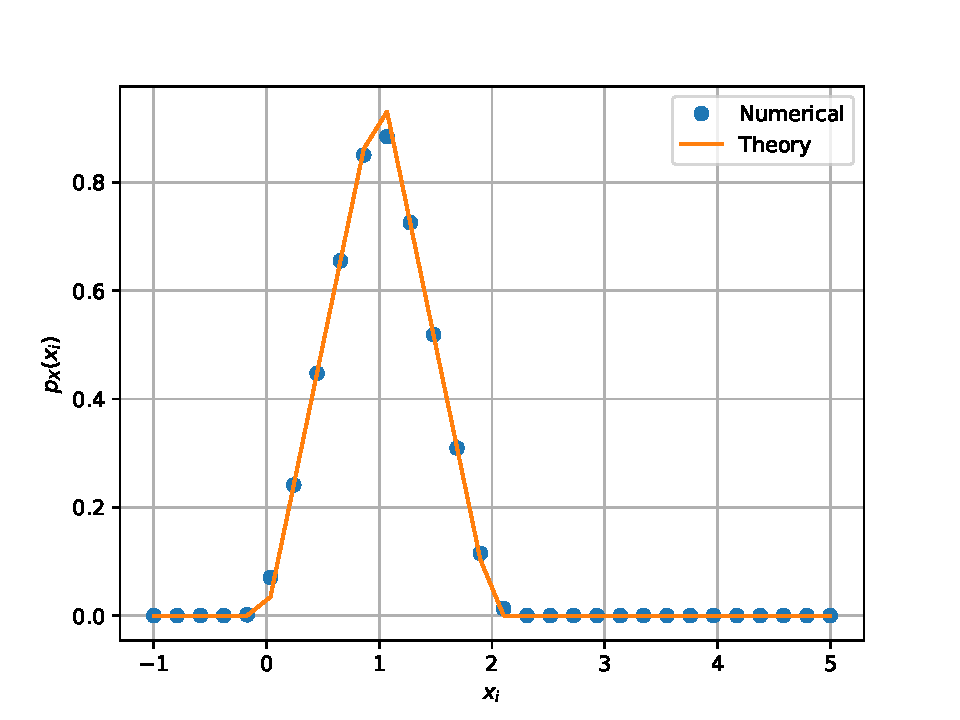
\includegraphics[width=\columnwidth]{./figs/chapter2/tri_pdf.pdf}
\caption{The PDF of $T$}
\label{fig:tri_pdf}
\end{figure}
\item Find the theoretical expressions for the PDF and CDF of $T$.\\
\solution Since $T$ is the sum of two independant random variables $U1$ and $U2$, the PDF of $T$ is given by
\begin{flalign}
	p_T(x) &= p_{U1}(x) \ast p_{U2}(x)
\end{flalign}
Using the PDF of $U$ from \eqref{eq:uni_pdf}, the convolution results in
\begin{align}
	p_T(x) &=
	\begin{cases}
		0 & x < 0\\
		x & 0 \le x \le 1\\
		2-x & 1 \le x \le 2\\
		0 & x > 2
	\end{cases}
	\label{eq:tri_pdf}
\end{align}
The CDF of $T$ is found using \eqref{eq:pdf_to_cdf} by replacing $U$ with $T$. Evaluating the integral for the piecewise function $p_T(x)$, 
\begin{align}
	F_T(x) &=
	\begin{cases}
		0 & x < 0\\
		\frac{x^2}{2} & 0 \le x \le 1\\
		2x-\frac{x^2}{2}-1 & 1 \le x \le 2\\
		1 & x > 2
	\end{cases}
\end{align}
\item Verify your results through a plot. \\
\solution The theoretical and numerical plots for the CDF and PDF of $T$ closely match in \figref{fig:tri_cdf} and \figref{fig:tri_pdf}
\end{enumerate}
\chapter{Maximum Likelihood Detection: BPSK}
\section{Maximum Likelihood}
\begin{enumerate}
\item Generate equiprobable $X \in \cbrak{1,-1}$.\\
\solution $X$ can be generated in python using the below code section,
\begin{lstlisting}[language=python]
import numpy as np	
num_samples = 500
x_var = np.random.choice([-1, 1], num_samples)
\end{lstlisting}
\item Generate 
\begin{equation}
Y = AX+N,
\end{equation}
		where $A = 5$ dB,  and $N \sim \gauss{0}{1}$.\\
\solution $Y$ can be generated in python using the below code section,
\begin{lstlisting}[language=python]
import numpy as np	
num_samples = 500
x_var = np.random.choice([-1, 1], num_samples)
n_var = np.random.normal(0, 1, num_samples)
A_db = 5
A = 10**(0.1*A_db)
y_var = A*x_var + n_var
\end{lstlisting}
\item Plot $Y$ using a scatter plot.\\
\solution The scatter plot of $Y$ is plotted in \figref{fig:bpsk_scatter} using the below code,
\begin{lstlisting}
codes/ch3/scatter.py
\end{lstlisting}
\begin{figure}[H]
\centering
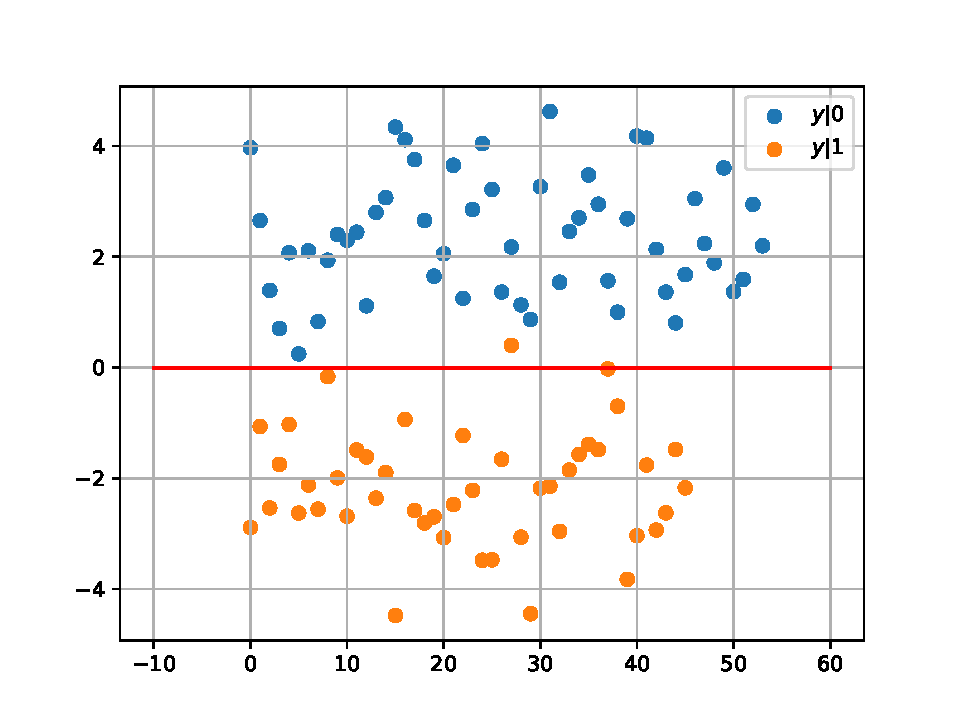
\includegraphics[width=\columnwidth]{./figs/chapter3/bpsk_scatter.pdf}
\caption{Scatter plot of $Y$}
\label{fig:bpsk_scatter}
\end{figure}
\item Guess how to estimate $X$ from $Y$.\\
\solution
\begin{equation}
y \dec{1}{-1} 0
\label{eq:bpsk_decision}
\end{equation}
\item
\label{ml-ch4_sim}
Find 
\begin{equation}
	P_{e|0} = \pr{\hat{X} = -1|X=1}
\end{equation}
and 
\begin{equation}
	P_{e|1} = \pr{\hat{X} = 1|X=-1}
\end{equation}\\
\solution Based on the decision rule in \eqref{eq:bpsk_decision},
\begin{flalign*}
	\pr{\hat{X} = -1|X=1} &= \pr{Y < 0|X=1}&\\
	&= \pr{AX + N < 0|X=1}&\\ 
	&= \pr{A + N < 0}&\\
	&= \pr{N < -A}
\end{flalign*}
Similarly,
\begin{flalign*}
	\pr{\hat{X} = 1|X=-1} &= \pr{Y > 0|X=-1}&\\
	&= \pr{N > A}
\end{flalign*}
Since $N \sim \gauss{0}{1}$,
\begin{flalign}
	\label{eq:std_norm_symmetric}
	\pr{N < -A} &= \pr{N > A}&\\
	\label{eq:bpks_prob_err_cond}
	\implies P_{e|0} &= P_{e|1} = \pr{N > A}
\end{flalign}
%
\item Find $P_e$ assuming that $X$ has equiprobable symbols.\\
\solution
\begin{flalign}
	P_e &= \pr{X=1}P_{e|1} + \pr{X=-1}P_{e|0}&\\
	\intertext{Since $X$ is equiprobable}\\
	\label{eq:bpsk_prob_error_equi}
	P_e &= \frac{1}{2}P_{e|1} + \frac{1}{2}P_{e|0}
\end{flalign}
Substituting from \eqref{eq:bpks_prob_err_cond}
\begin{equation}
	P_e = \pr{N > A}
\end{equation}
Given a random varible $X \sim \gauss{0}{1}$ the Q-function is defined as
\begin{align}
	Q(x) &= \pr{X > x}\\
	\label{eq:q_func_integral}
	Q(x) &= \frac{1}{\sqrt{2\pi}} \int_x^\infty \exp\left(-\frac{u^2}{2}\right) \, du.\\
\end{align}
Using the Q-function, $P_e$ is rewritten as
\begin{equation}
	P_e = Q(A)
\end{equation} 
%
\item
Verify by plotting  the theoretical $P_e$ with respect to $A$ from 0 to 10 dB.\\
\solution The theoretical $P_e$ is plotted in \figref{fig:bpsk_pe_snr}, along with numerical estimations from generated samples of $Y$. The below code is used for the plot, 
\begin{lstlisting}
codes/ch3/bpsk_pe.py
\end{lstlisting}
\begin{figure}[H]
\centering
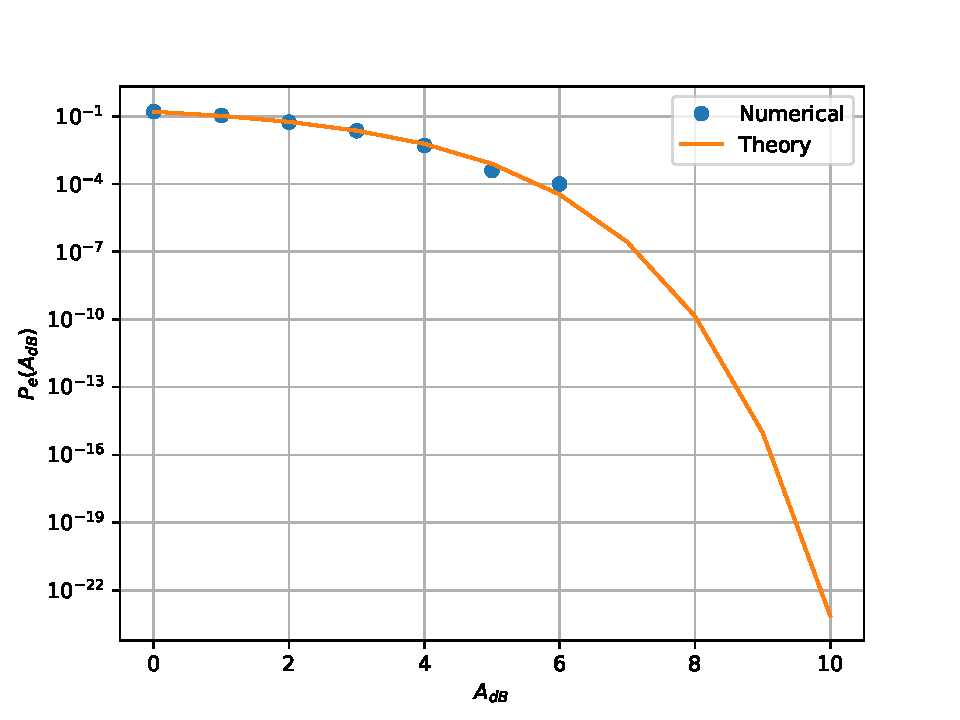
\includegraphics[width=\columnwidth]{./figs/chapter3/bpsk_pe_snr.pdf}
\caption{$P_e$ versus $A$ plot}
\label{fig:bpsk_pe_snr}
\end{figure}
%
\item Now, consider a threshold $\delta$  while estimating $X$ from $Y$. Find the value of $\delta$ that maximizes the theoretical $P_e$.\\
\label{prob:bpsk_delta_equi}
\solution Given the decision rule, 
\begin{equation}
y \dec{1}{-1} \delta
\label{eq:bpsk_decision_delta}
\end{equation}
\begin{flalign*}
	P_{e|0} &= \pr{\hat{X} = -1|X=1}&\\
	&= \pr{Y < \delta|X=1}&\\
	&= \pr{AX + N < \delta|X=1}&\\ 
	&= \pr{A + N < \delta}&\\
	&= \pr{N < -A + \delta}&\\
	&= \pr{N > A - \delta}&\\
	&= Q(A-\delta)
\end{flalign*}
\begin{flalign*}
	P_{e|1} &= \pr{\hat{X} = 1|X=-1}&\\
	&= \pr{Y > \delta|X=-1}&\\
	&= \pr{N > A + \delta}&\\
	&= Q(A+\delta)
\end{flalign*}
Using \eqref{eq:bpsk_prob_error_equi}, $P_e$ is given by
\begin{flalign}
	P_e &= \frac{1}{2}Q(A+\delta) + \frac{1}{2}Q(A-\delta)
\end{flalign}
Using the integral for Q-function from \eqref{eq:q_func_integral},
\begin{align}
	\label{eq:prob_error_delta_equi}
	P_e &= k(\int_{A+\delta}^\infty \exp\left(-\frac{u^2}{2}\right) \, du + \int_{A-\delta}^\infty \exp\left(-\frac{u^2}{2}\right) \, du)\\
	\intertext{where k is a constant}	\nonumber
\end{align}
Differentiating \eqref{eq:prob_error_delta_equi} wrt $\delta$ (using Leibniz's rule) and equating to $0$, we get
\begin{flalign*}
	\exp\left(-\frac{(A+\delta)^2}{2}\right)-\exp\left(-\frac{(A-\delta)^2}{2}\right) &= 0&\\
	\frac{\exp\left(-\frac{(A+\delta)^2}{2}\right)}{\exp\left(-\frac{(A-\delta)^2}{2}\right)} &= 1&\\
	\exp\left(-\frac{(A+\delta)^2-(A-\delta)^2}{2}\right) &= 1&\\
	\exp\left(-2A\delta\right) &= 1&\\
	\intertext{Taking $\ln$ on both sides}\\
	-2A\delta &= 0&\\
	\implies \delta &= 0
\end{flalign*}
$P_e$ is maximum for $\delta = 0$
\item Repeat the above exercise when 
\label{prob:bpsk_decision_uneqi}
	\begin{align}
		p_{X}(0) = p
	\end{align}\\
\solution Since $X$ is not equiprobable, $P_e$ is given by,
\begin{flalign}
	P_e &= (1-p)P_{e|1} + pP_{e|0}&\\
	&= (1-p)Q(A+\delta) + pQ(A-\delta)
\end{flalign}
Using the integral for Q-function from \eqref{eq:q_func_integral},
\begin{multline}
	\label{eq:prob_error_delta_nonequi}
	P_e = k((1-p)\int_{A+\delta}^\infty \exp\left(-\frac{u^2}{2}\right) \, du + \\
	p\int_{A-\delta}^\infty \exp\left(-\frac{u^2}{2}\right) \, du)
\end{multline}
where $k$ is a constant.\\
Following the same steps as in problem \ref{prob:bpsk_delta_equi}, $\delta$ for maximum $P_e$ evaluates to,
\begin{equation}
	\delta = \frac{1}{2A}\ln\left(\frac{1}{p}-1\right)
\end{equation}
\item Repeat the above exercise using the MAP criterion.\\
\solution 
The MAP rule can be stated as\\
\begin{flalign}
\text{Set } \hat{x} &= x_i \text{ if}&\\ \nonumber
p_X(x_k)p_Y(y|x_k) &\text{ is maximum for } k = i
\end{flalign}
For the case of BPSK, the point of equality between $p_X(x=1)p_Y(y|x=1)$ and $p_X(x=-1)p_Y(y|x=-1)$ is the optimum threshold. If this threshold is $\delta$, then
\begin{flalign*}
	pp_Y(y|x=1) > (1-p)p_Y(y|x=-1) &\text{ when } y > \delta&\\
	pp_Y(y|x=1) < (1-p)p_Y(y|x=-1) &\text{ when } y < \delta 	
\end{flalign*}
The above inequalities can be visualized in \figref{fig:bpsk_map_density} for $p = 0.3$ and $A = 3$.
\begin{figure}[H]
\centering
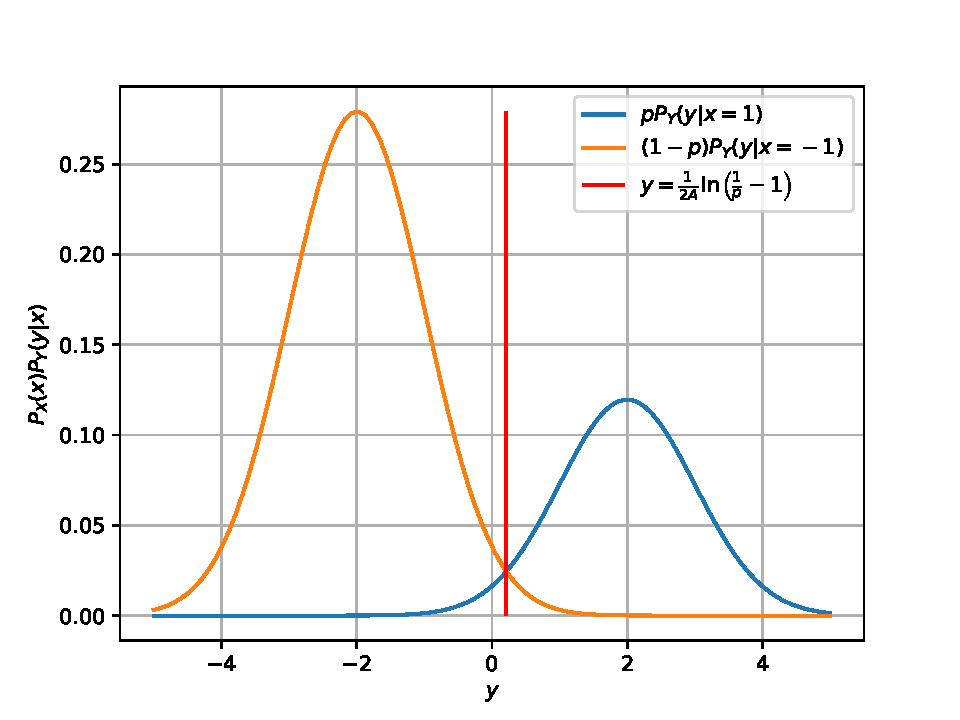
\includegraphics[width=\columnwidth]{./figs/chapter3/bpsk_map_density.pdf}
\caption{$p_X(X=x_i)p_Y(y|x=x_i)$ versus $y$ plot for $X \in \{-1,1\}$}
\label{fig:bpsk_map_density}
\end{figure}
Given $Y=AX+N$ where $N \sim \gauss{0}{1}$, the optimum threshold is found as solution to the below equation
\begin{equation}
	p\exp\left(-\frac{(y_{eq}-A)^2}{2}\right) = (1-p)\exp\left(-\frac{(y_{eq}+A)^2}{2}\right)
\end{equation}
Solving for $y_{eq}$, we get
\begin{equation}
	y_{eq} = \delta = \frac{1}{2A}\ln\left(\frac{1}{p}-1\right)
\end{equation}
which is same as $\delta$ obtained in problem \ref{prob:bpsk_decision_uneqi}

\end{enumerate}
\chapter{Transformation of Random Variables}
\section{Gaussian to Other}
\begin{enumerate}
\item
Let $X_1 \sim  \gauss{0}{1}$ and $X_2 \sim  \gauss{0}{1}$. Plot the CDF and PDF of
%
\begin{equation}
V = X_1^2 + X_2^2
\end{equation}\\
\solution The CDF and PDF of $V$ are plotted in \figref{fig:chisq_cdf} and \figref{fig:chisq_pdf} respectively using the below code
\begin{lstlisting}
codes/ch4/sum_of_squares.py
\end{lstlisting}
\begin{figure}[H]
\centering
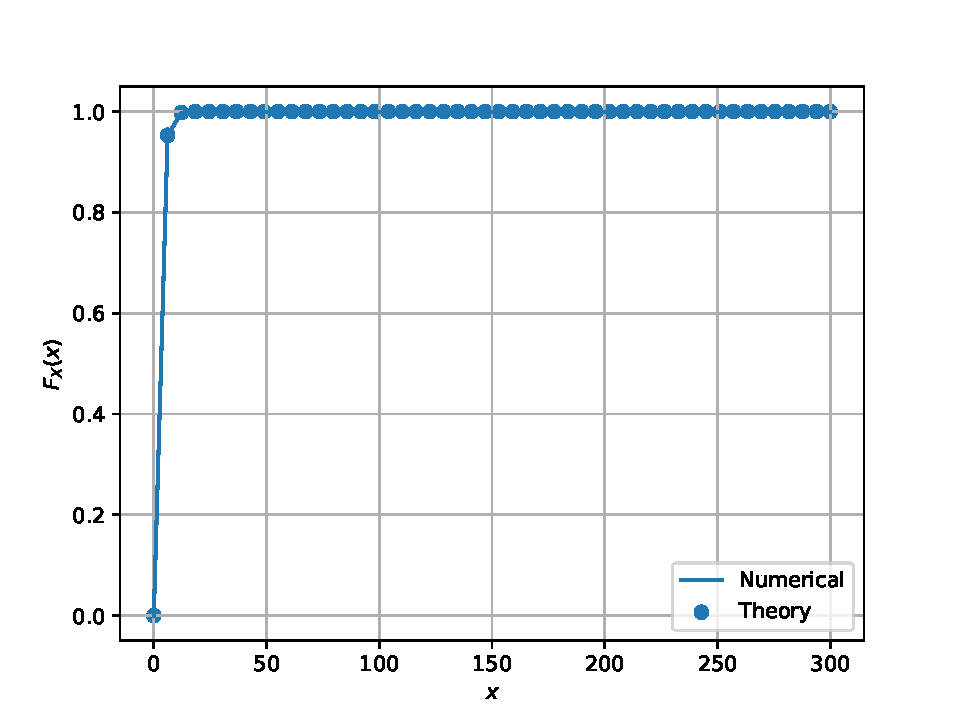
\includegraphics[width=\columnwidth]{./figs/chapter4/chisq_cdf.pdf}
\caption{CDF of $V$}
\label{fig:chisq_cdf}
\end{figure}
\begin{figure}[H]
\centering
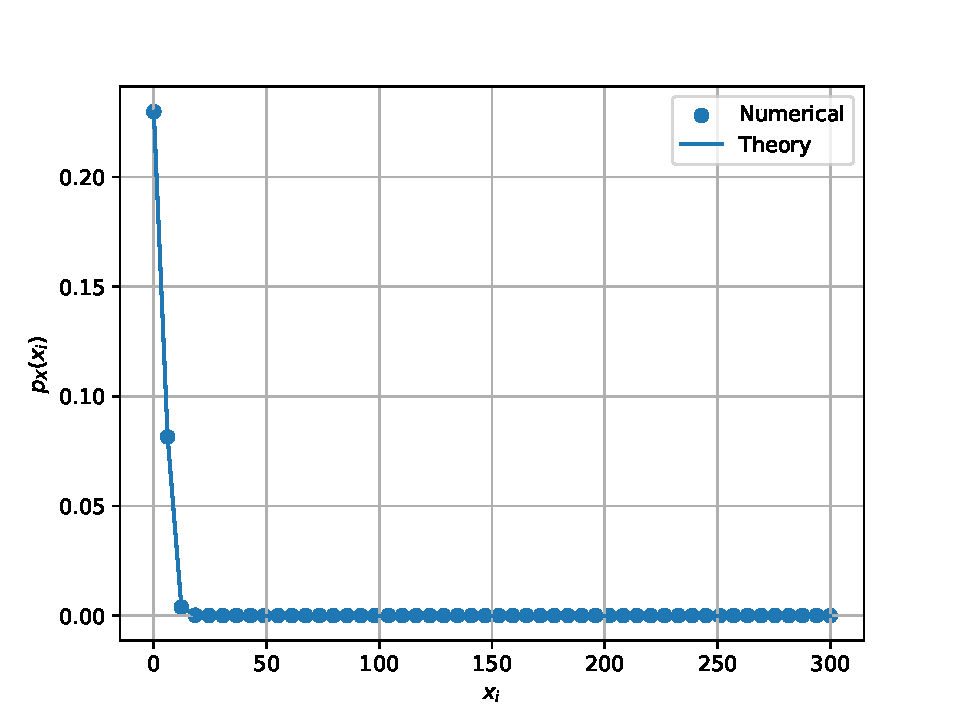
\includegraphics[width=\columnwidth]{./figs/chapter4/chisq_pdf.pdf}
\caption{PDF of $V$}
\label{fig:chisq_pdf}
\end{figure}
%

%
%
\item
If
%
\begin{equation}
F_{V}(x) = 
\begin{cases}
1 - e^{-\alpha x} & x \geq 0 \\
0 & x < 0,
\end{cases}
\end{equation}
%
find $\alpha$.\\
\solution Let $Z=X^2$ where $X \sim \gauss{0}{1}$. Defining the CDF for $Z$,
\begin{flalign*}
	P_Z(z) &= \pr{Z < z}&\\
	&= \pr{X^2 < z}&\\
	&= \pr{-\sqrt{z} < X < \sqrt{z}}&\\
	&= \int_{-\sqrt{z}}^{\sqrt{z}} p_X(x)  \,dx 
\end{flalign*}
Using \eqref{eq:cdf_to_pdf}, the PDF of $Z$ is given by
\begin{align}
	\nonumber
	\frac{d}{dz}P_Z(z) &= p_Z(z)\\
	\label{eq:square_pdf_gen}
	= \frac{p_X(\sqrt{z})+p_X(-\sqrt{z})}{2\sqrt{z}} & \text{ (Using Lebniz's rule)} 
\end{align}
Substituting the standard gaussian density function $p_X(x) = \frac{1}{\sqrt{2\pi}}e^{-\frac{x^2}{2}}$ in \eqref{eq:square_pdf_gen},
\begin{equation}
	p_Z(z) =
	\begin{cases}
	\frac{1}{\sqrt{2\pi z}}e^{-\frac{z}{2}} & z \ge 0\\
	0 & z < 0
	\end{cases} 
	\label{eq:chisq_pdf}
\end{equation}
The PDF of $X_1^2$ and $X_2^2$ are given by \eqref{eq:chisq_pdf}. Since $V$ is the sum of two independant random variables,
\begin{flalign*}
	p_V(v) &= p_{X_1^2}(x_1) \ast p_{X_2^2}(x_2)&\\
	&= \frac{1}{2\pi} \int_{0}^{v} \frac{e^{-\frac{x}{2}}}{\sqrt{x}}\frac{e^{-\frac{v-x}{2}}}{\sqrt{v-x}}  \,dx&\\
	&= \frac{e^{-\frac{v}{2}}}{2\pi} \int_{0}^{v} \frac{1}{\sqrt{x(v-x)}}  \,dx&\\
	&= \frac{e^{-\frac{v}{2}}}{2\pi} \sbrak{-\arcsin\left(\dfrac{v-2x}{v}\right)}_0^v&\\
	&= \frac{e^{-\frac{v}{2}}}{2\pi} \pi&\\
	&= \frac{e^{-\frac{v}{2}}}{2} \text{ for } v \ge 0
\end{flalign*}
$F_V(v)$ can be obtained from $p_V(v)$ using \eqref{eq:pdf_to_cdf}
\begin{flalign}
	\nonumber
	F_V(v) &= \frac{1}{2} \int_{0}^{v} \exp\left(-\frac{v}{2}\right)&\\
	\label{eq:chisq2_cdf}
	&= 1-\exp\left(-\frac{v}{2}\right) \text{ for } v \ge 0
\end{flalign}
Comparing \eqref{eq:chisq2_cdf} with \eqref{eq:chisq2_cdf_gen}, $\alpha = \frac{1}{2}$ 
%
\item
\label{ch3_raleigh_sim}
Plot the CDF and PDF of
%
\begin{equation}
A = \sqrt{V}
\end{equation}\\
\solution The CDF and PDF of $A$ are plotted in \figref{fig:rayleigh_cdf} and \figref{fig:rayleigh_pdf} respectively using the below code
\begin{lstlisting}
codes/ch4/square_root.py
\end{lstlisting}
The CDF of $A$ is given by,
\begin{align}
	F_{A}\brak{a} &= \pr{A < a}\\
	&= \pr{\sqrt{V} < a}\\
	&= \pr{V < a^2}\\
	&= F_{V}\brak{a^2}\\
	&= 1-\exp\brak{-\frac{a^2}{2}} 
\end{align}
Using \eqref{eq:cdf_to_pdf}, the PDF is found to be
\begin{align}
	p_{A}\brak{a} &= a\exp\brak{-\frac{a^2}{2}}
\end{align}
\begin{figure}[H]
\centering
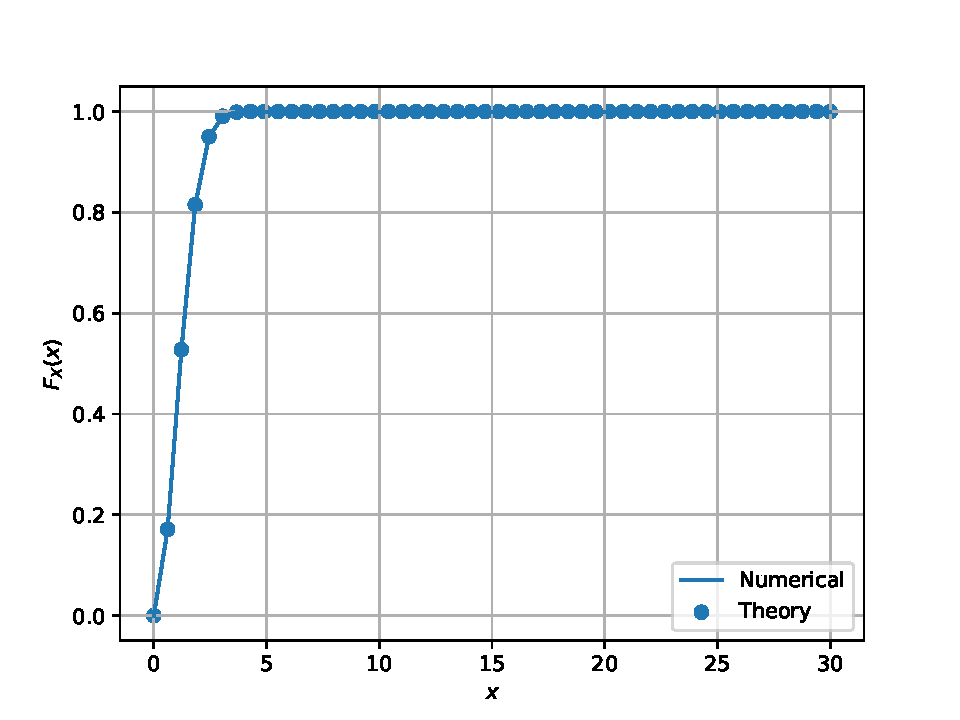
\includegraphics[width=\columnwidth]{./figs/chapter4/rayleigh_cdf.pdf}
\caption{CDF of $A$}
\label{fig:rayleigh_cdf}
\end{figure}
\begin{figure}[H]
\centering
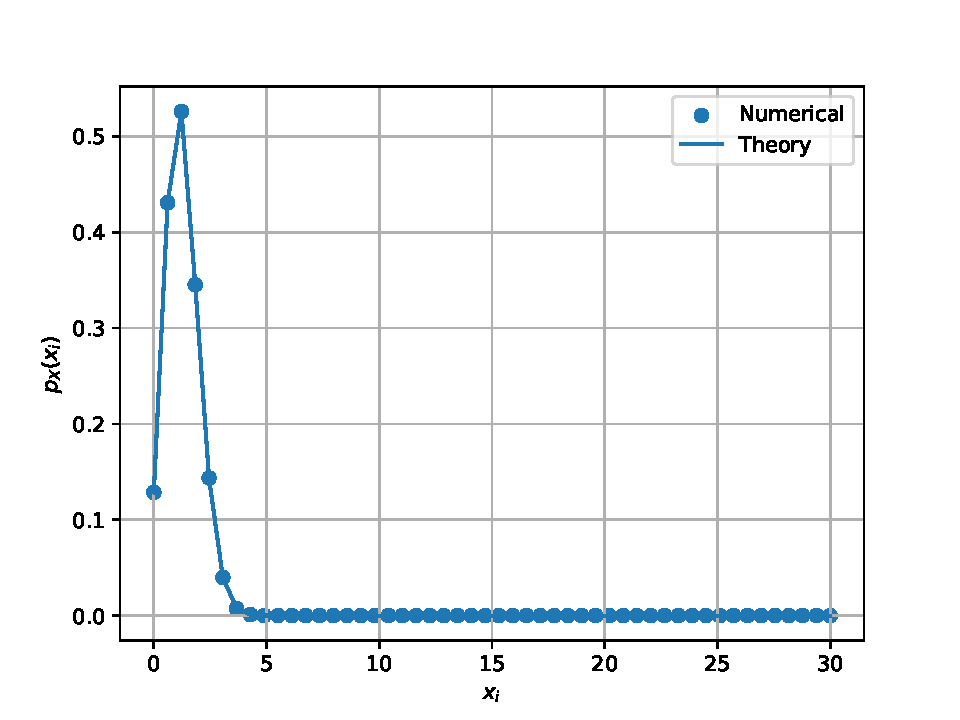
\includegraphics[width=\columnwidth]{./figs/chapter4/rayleigh_pdf.pdf}
\caption{PDF of $A$}
\label{fig:rayleigh_pdf}
\end{figure}
%


\end{enumerate}

\section{Conditional Probability}
\begin{enumerate}
\item
\label{ch4_sim}
Plot 
\begin{equation}
P_e = \pr{\hat{X} = -1|X=1}
\end{equation}
%
for 
\begin{equation}
Y = AX+N,
\end{equation}
where $A$ is Raleigh with $E\sbrak{A^2} = \gamma, N \sim \gauss{0}{1}, X \in \brak{-1,1}$ for $0 \le \gamma \le 10$ dB.\\
\solution The blue dots in \figref{fig:bpsk_pe_snr_rayleigh} is the required plot. The below code is used to generate the plot,
\begin{lstlisting}
codes/ch4/prob_error.py
\end{lstlisting}
%
\item
Assuming that $N$ is a constant, find an expression for $P_e$.  Call this $P_e(N)$\\
\solution Assuming the decision rule in \eqref{eq:bpsk_decision}, when $N$ is constant, $P_e$ is given by 
\begin{flalign}
	\nonumber
	P_e &= \pr{\hat{X} = -1|X=1}&\\ \nonumber
	&= \pr{Y<0|X=1}&\\ \nonumber
	&= \pr{AX+N<0|X=1}&\\ 
	\label{eq:prob_err_rayleigh_gen}
	&= \pr{A+N<0}&\\ \nonumber
	&= \pr{A<-N}&\\
	\label{eq:prob_err_bpsk_rayleigh_cdf}
	&=
	\begin{cases}
	F_A(-N) & N \ge 0\\
	0 & N < 0
	\end{cases}
\end{flalign}
For a Rayleigh random variable $X$ with $E\sbrak{X^2} = \gamma$, the PDF and CDF are given by
\begin{align}
	\label{eq:rayleigh_pdf}
	p_X(x) &= \frac{2x}{\gamma}\exp\left(-\frac{x^2}{\gamma}\right) \text{ for } x \ge 0\\
	\label{eq:rayleigh_cdf}
	F_X(X) &= 1-\exp\left(-\frac{x^2}{\gamma}\right) \text{ for } x \ge 0
\end{align}
Substituting \eqref{eq:rayleigh_cdf} in \eqref{eq:prob_err_bpsk_rayleigh_cdf},
\begin{equation}
	\label{eq:prob_err_bpsk_rayleigh_fN}
	P_e(N) =
	\begin{cases} 
	1-\exp\left(-\frac{N^2}{\gamma}\right) & N \ge 0\\
	0 & N < 0
	\end{cases}
\end{equation}
%
\item
%
\label{ch4_anal}
For a function $g$,
\begin{equation}
E\sbrak{g(X)} = \int_{-\infty}^{\infty}g(x)p_{X}(x)\, dx
\end{equation}
%
Find $P_e = E\sbrak{P_e(N)}$.\\
\solution Using $P_e(N)$ from \eqref{eq:prob_err_bpsk_rayleigh_fN},
\begin{flalign*}
	P_e &= \int_{-\infty}^{\infty} P_e(x)p_N(x) \,dx&\\
	&= \int_{0}^{\infty} \left(1-e^{-\frac{x^2}{\gamma}}\right)\frac{1}{\sqrt{2\pi}}e^{-\frac{x^2}{2}} \,dx
\end{flalign*}
	
\begin{multline*}
	P_e = \frac{1}{\sqrt{2\pi}}\int_{0}^{\infty} e^{-\frac{x^2}{2}}  \,dx \\ - \frac{1}{\sqrt{2\pi}}\int_{0}^{\infty} \exp\left(-x^2\left(\frac{1}{\gamma}+\frac{1}{2}\right)\right)  \,dx
\end{multline*}
\begin{flalign*}
	P_e &= \frac{1}{2} - \frac{1}{2}\sqrt{\frac{\gamma}{2+\gamma}}
\end{flalign*} 
%
\item
Plot $P_e$ in problems \ref{ch4_sim} and \ref{ch4_anal} on the same graph w.r.t $\gamma$.  Comment.\\
\solution $P_e$ plotted in same graph in \figref{fig:bpsk_pe_snr_rayleigh}. The value of $P_e$ is much higher when the channel %
gain $A$ is Rayleigh distributed than the case where $A$ is a constant (compare with \figref{fig:bpsk_pe_snr}).
\begin{figure}[H]
\centering
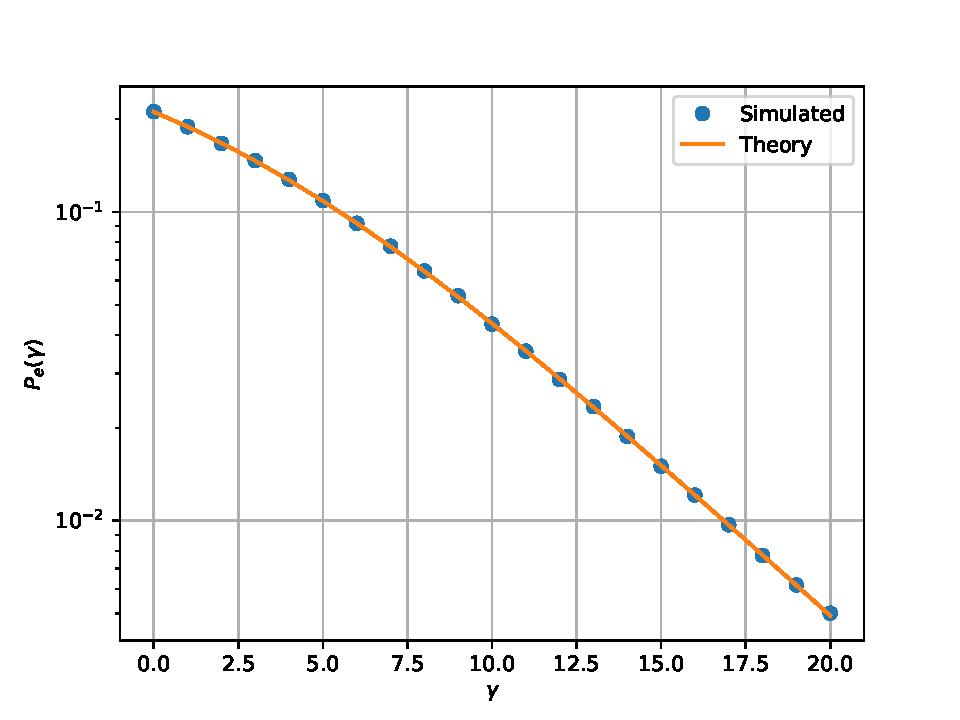
\includegraphics[width=\columnwidth]{./figs/chapter4/prob_error.pdf}
\caption{$P_e$ versus $\gamma$}
\label{fig:bpsk_pe_snr_rayleigh}
\end{figure}
From \eqref{eq:prob_err_rayleigh_gen}, $P_e$ is given by
\begin{equation}
	P_e = \pr{A+N<0}
\end{equation}
One method of computing \eqref{eq:prob_err_rayleigh_gen} is by finding the PDF of $Z=A+N$ (as the convolution of the individual PDFs of %
$A$ and $N$) and then integrating $p_Z(z)$ from $-\infty$ to $0$. The other method is by first computing $P_e$ for constant $N$ and then finding %
the expectation of $P_e(N)$. Both provide the same result but the computation of integrals is simpler when using the latter method. 

\end{enumerate}
\chapter{Bivariate Random Variables: FSK}
\section{Two Dimensions}
Let 
\begin{equation}
\mbf{y} = A\mbf{x} + \mbf{n},
\end{equation}
where 
\begin{align}
x &\in \brak{\mbf{s}_0,\mbf{s}_1}, 
\mbf{s}_0 = 
\begin{pmatrix}
1 
\\
0
\end{pmatrix},
\mbf{s}_1 = 
\begin{pmatrix}
0 
\\
1
\end{pmatrix}
\\
\mbf{n} &= 
\begin{pmatrix}
n_1
\\
n_2
\end{pmatrix},
n_1,n_2 \sim \gauss{0}{1}.
\end{align}
%
\begin{enumerate}
%%
\item
\label{ch5_fsk}
Plot 
%
\begin{equation}
\mbf{y}|\mbf{s}_0 \text{ and } \mbf{y}|\mbf{s}_1
\end{equation}
%
on the same graph using a scatter plot.\\
\solution The scatter plot in \figref{fig:biv_scatter} is generated using the below code,
\begin{lstlisting}
codes/ch5/biv_scatter.py
\end{lstlisting}
%
\begin{figure}[H]
\centering
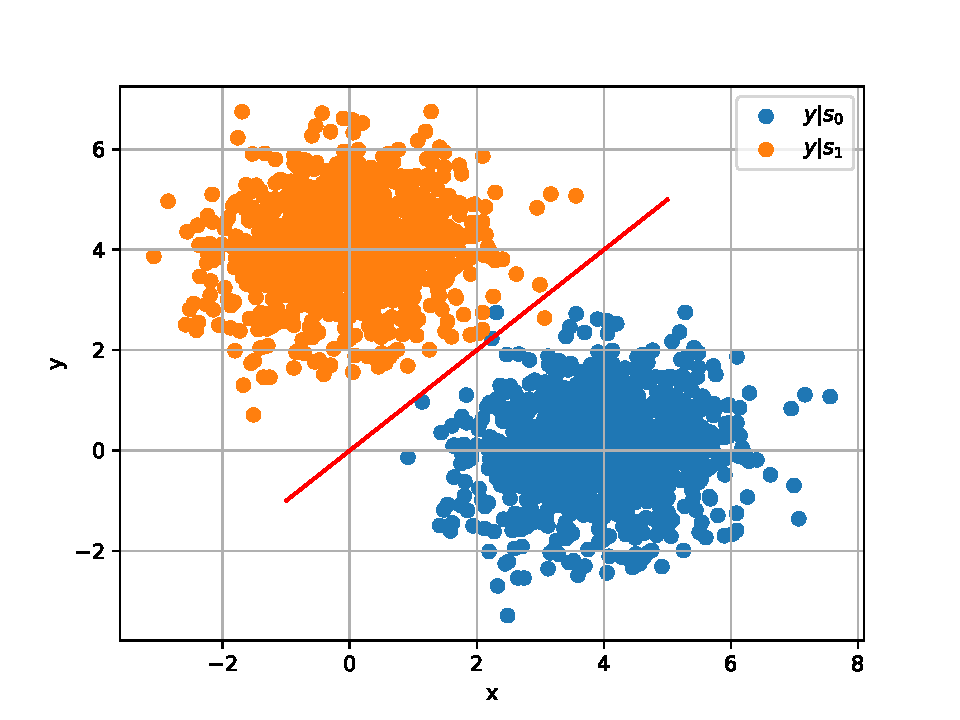
\includegraphics[width=\columnwidth]{./figs/chapter5/biv_scatter.pdf}
\caption{Scatter plot of $\mbf{y}|\mbf{s}_0$ and $\mbf{y}|\mbf{s}_1$ }
\label{fig:biv_scatter}
\end{figure}

%
\item
For the above problem, find a decision rule for detecting the symbols $\mbf{s}_0 $ and $\mbf{s}_1$.\\
\solution Let $\mbf{y} = \myvec{y_1&y_2}^T$. Then the decision rule is
\begin{equation}
	y_1 \dec{0}{1} y_2
	\label{eq:biv_fsk_decision}
\end{equation}
\begin{equation}
	p_{\vec{y}|\vec{s}_i}\brak{\vec{y}} = \frac{1}{2\pi\sqrt{\mydet{\vec{\Sigma}}}} \exp\brak{-\frac{1}{2}\brak{\vec{y}-\vec{s}_i}^\top \vec{\Sigma}^{-1} \brak{\vec{y}-\vec{s}_i}}
\end{equation}
Where $\vec{\Sigma}$ is the covariance matrix. Substituting $\vec{\Sigma} = \sigma \vec{I}$,
\begin{align}
	p_{\vec{y}|\vec{s}_i}\brak{\vec{y}} &= \frac{1}{2 \pi \sigma} \exp\brak{-\frac{1}{2 \sigma}\brak{\vec{y}-\vec{s}_i}^\top \vec{I} \brak{\vec{y}-\vec{s}_i}}\\
	&= \frac{1}{2 \pi \sigma} \exp\brak{-\frac{1}{2 \sigma}\brak{\vec{y}-\vec{s}_i}^\top \brak{\vec{y}-\vec{s}_i}}
\end{align}
Assuming equiprobable symbols, use MAP rule to find optimum decision. Since there are only two possible symbols %
$\vec{s}_0$ and $\vec{s}_1$, the optimal decision criterion is found by equating $p_{\vec{y}|\vec{s}_0}$ and $p_{\vec{y}|\vec{s}_1}$.
\begin{align*}
	p_{\vec{y}|\vec{s}_0} &= p_{\vec{y}|\vec{s}_1}
\end{align*}
	
\begin{multline*}
	\implies \exp\brak{-\frac{1}{2 \sigma}\brak{\vec{y}-\vec{s}_0}^\top \brak{\vec{y}-\vec{s}_0}} = \\
	\exp\brak{-\frac{1}{2 \sigma}\brak{\vec{y}-\vec{s}_1}^\top \brak{\vec{y}-\vec{s}_1}}
\end{multline*}
	
\begin{align*}
	\implies \brak{\vec{y}-\vec{s}_0}^\top \brak{\vec{y}-\vec{s}_0} &= \brak{\vec{y}-\vec{s}_1}^\top \brak{\vec{y}-\vec{s}_1}\\
	\implies \vec{y}^\top\vec{y} - 2\vec{s}_0^\top \vec{y} + \vec{s}_0^T\vec{s}_0 &= \vec{y}^\top\vec{y} - 2\vec{s}_1^\top \vec{y} + \vec{s}_1^T\vec{s}_1\\
	\implies 2\brak{\vec{s}_1-\vec{s}_0}^\top \vec{y} &= \norm{\vec{s}_1}^2 - \norm{\vec{s}_0}^2\\
	\implies \brak{\vec{s}_1-\vec{s}_0}^\top \vec{y} &= 0\\
	\implies \myvec{-1\\1}^\top \vec{y} &= 0
\end{align*}
%
%
\item
Plot 
\begin{equation} 
P_e = \pr{\hat{\mbf{x}} = \mbf{s}_1|\mbf{x} = \mbf{s}_0}
\label{eq:prob_error_fsk}
\end{equation}
with respect to the SNR from 0 to 10 dB.\\
\solution The blue dots in \figref{fig:biv_pe_snr} are the $P_e$ versus SNR plot. It is generated using the below code,
\begin{lstlisting}
codes/ch5/biv_pe_snr.py
\end{lstlisting}
%
\item
Obtain an expression for $P_e$. Verify this by comparing the theory and simulation plots on the same graph.\\
\solution Using the decision rule from \eqref{eq:biv_fsk_decision},
\begin{align}
	\nonumber
	P_e &= \pr{\hat{\mbf{x}} = \mbf{s}_1|\mbf{x} = \mbf{s}_0}\\\nonumber
	&= \pr{y_1 < y_2|\mbf{x} = \mbf{s}_0}\\\nonumber
	&= \pr{A+n_1 < n_2}\\
	\label{eq:prob_error_fsk_inter}
	&= \pr{n_1-n_2 < -A}
\end{align}
Let $Z = n_1-n_2$ where $n_1, n_2 \sim \gauss{0}{\sigma^2}$. The PDF of X is given by,
\begin{align}
	\nonumber
	p_Z(z) &= p_{n_1}(n_1) \ast p_{-n_2}(n_2)\\\nonumber
	&= \frac{1}{2\pi\sigma^2}\int_{-\infty}^{\infty} e^{-\frac{t^2}{2\sigma^2}}e^{-\frac{(t-z)^2}{2\sigma^2}}  \,dt\\\nonumber
	&= \frac{1}{2\pi\sigma^2}\int_{-\infty}^{\infty} e^{-\frac{(z-t)^2+t^2}{2\sigma^2}}  \,dt\\\nonumber
	&= \frac{1}{2\pi\sigma^2}\int_{-\infty}^{\infty} e^{-\frac{(2t-z)^2+z^2}{2(\sqrt{2}\sigma)^2}}  \,dt\\\nonumber
	&= \frac{1}{2\pi\sigma^2}e^{-\frac{z^2}{2(\sqrt{2}\sigma)^2}}\int_{-\infty}^{\infty} e^{-\frac{(2t-z)^2}{2(\sqrt{2}\sigma)^2}}  \,dt\\\nonumber
	&= \frac{e^{-\frac{z^2}{2(\sqrt{2}\sigma)^2}}}{\sqrt{2\pi}\sqrt{2}\sigma} \frac{1}{\sqrt{2\pi}\sqrt{2}\sigma}\int_{-\infty}^{\infty} e^{-\frac{k^2}{2(\sqrt{2}\sigma)^2}}  \,dk\\
	\label{eq:std_gauss_diff_pdf_fsk}
	&= \frac{e^{-\frac{z^2}{2(\sqrt{2}\sigma)^2}}}{\sqrt{2\pi}\sqrt{2}\sigma}
\end{align}
From \eqref{eq:std_gauss_diff_pdf_fsk}, $Z \sim \gauss{0}{2\sigma^2}$. Substituting $\sigma=1$, $Z \sim \gauss{0}{2}$. %
\eqref{eq:prob_error_fsk_inter} can be further simplified as,
\begin{align*}
	P_e &= \pr{Z < -A}&\\
	&= \pr{Z > A}&\\
	&= \qfunc{\frac{A}{\sqrt{2}}}&\\
	&= \frac{1}{\sqrt{2\pi}}\int_{\frac{A}{\sqrt{2}}}^{\infty} \exp\left(-\frac{x^2}{2}\right)  \,dx 
\end{align*}
\figref{fig:biv_pe_snr} compares the theoretical and simulation plots

\begin{figure}[H]
\centering
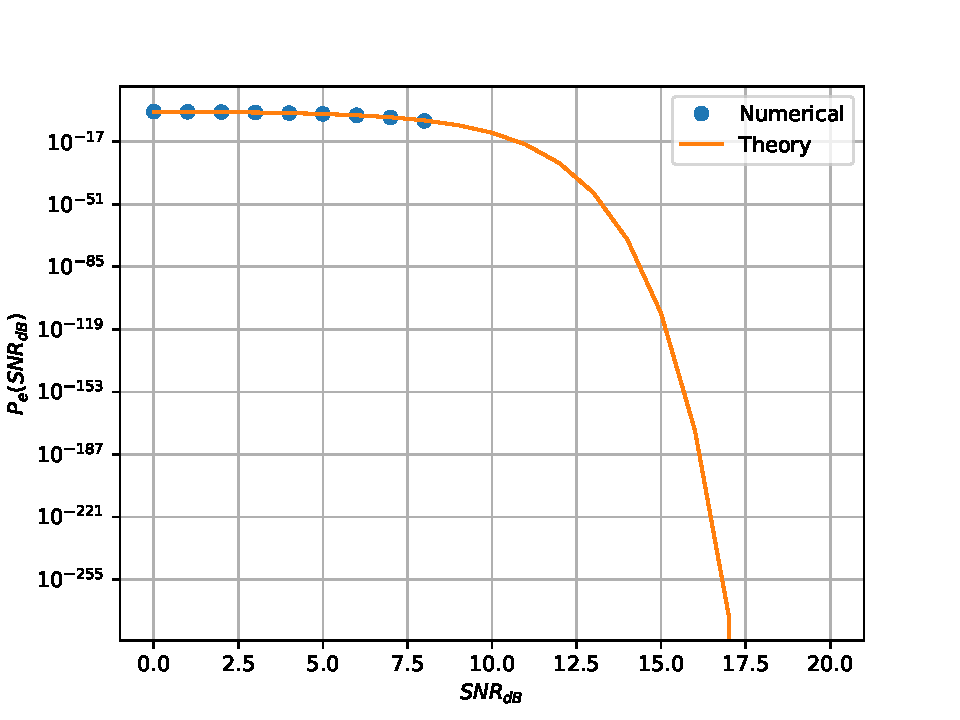
\includegraphics[width=\columnwidth]{./figs/chapter5/biv_pe_vs_snr.pdf}
\caption{$P_e$ versus SNR plot for FSK}
\label{fig:biv_pe_snr}
\end{figure}
%
\end{enumerate}

\chapter{Exercises}
\section{BPSK}
\begin{enumerate}
\item
The {\em signal constellation diagram} for BPSK is given by Fig. \ref{fig:bpsk_const}.  The symbols $s_0$ and $s_1$ are equiprobable.  $\sqrt{E_b}$ is the energy transmitted per bit. Assuming a zero mean additive white gaussian noise (AWGN) with variance $\frac{N_0}{2}$,
obtain the symbols that are received.

%
\begin{figure}[H]
\centering
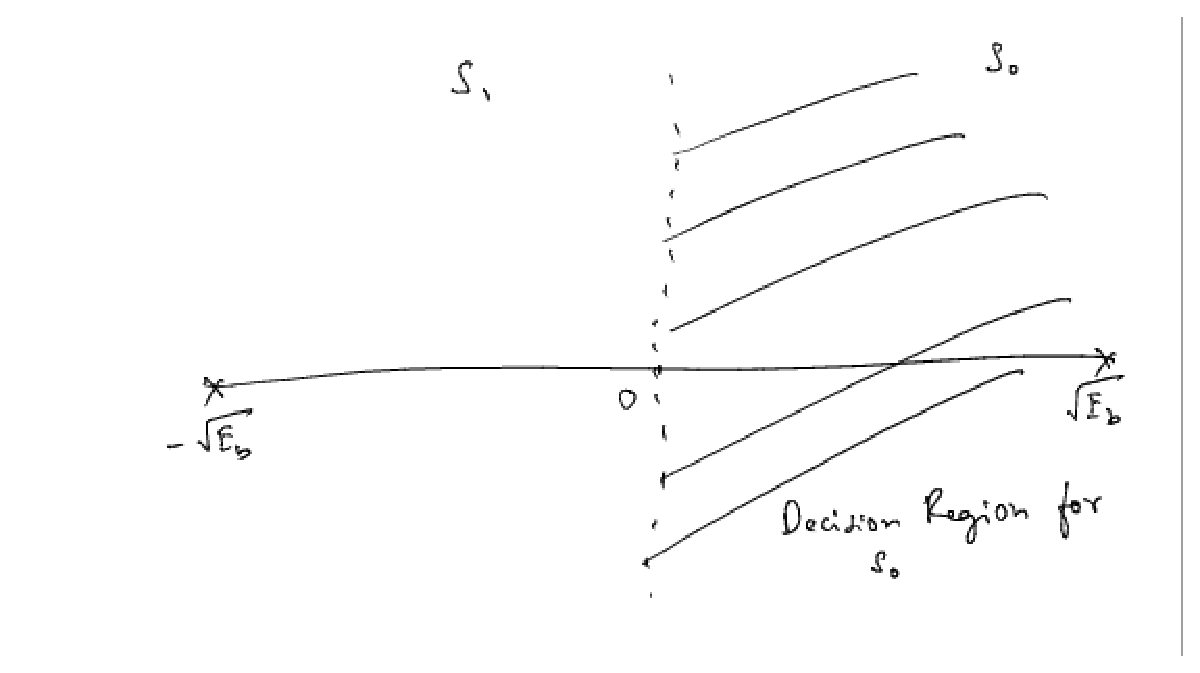
\includegraphics[width=\columnwidth]{./figs/chapter6/bpsk_const.eps}
\caption{}
\label{fig:bpsk_const}
\end{figure}
\solution The possible received symbols are
\begin{align}
y|s_0 &= \sqrt{E_b} + n
\\
y|s_1 &= -\sqrt{E_b} + n
\end{align}
%
where the AWGN $n \sim \gauss{0}{\frac{N_0}{2}}$.
%
\item
\label{prob:bpsk_decision}
From Fig. \ref{fig:bpsk_const} obtain a decision rule for BPSK

\solution The decision rule is
\begin{equation}
y \dec{s_0}{s_1} 0
\end{equation}
\item
Repeat the previous exercise using the MAP criterion.\\
\solution When the symbols are equiprobable, the MAP rule stated in \eqref{eq:map_rule} simplifies to finding the symbol $s_i$ that %
maximizes the conditional PDF $p_Y(y|s_i)$ i.e.
\begin{align}
	\label{eq:mle_rule}
	\text{Set } \hat{x} &= x_i \text{ if}&\\ \nonumber
	p_Y(y|x_k) &\text{ is maximum for } k = i
\end{align}
In the case of BPSK, $y|s_0 \sim \gauss{\sqrt{E_b}}{\frac{N_0}{2}}$ and $y|s_1 \sim \gauss{-\sqrt{E_b}}{\frac{N_0}{2}}$. %
The two PDFs meet at $Y=0$. So,
\begin{align*}
	p_Y(y|s_0) > p_Y(y|s_1) &\text{ when } y > 0&\\
	p_Y(y|s_0) < p_Y(y|s_1) &\text{ when } y < 0 	
\end{align*}
The optimum threshold is therefore $Y=0$

\item
Using the decision rule in Problem \ref{prob:bpsk_decision}, obtain an expression for the probability of error for BPSK.
\solution
Since the symbols are equiprobable, it is sufficient if the error is calculated assuming that a 0 was sent.  This results in
\begin{align}
P_e &= \pr{y < 0|s_0} = \pr{\sqrt{E_b} + n < 0}
\\
&= \pr{ -n > \sqrt{E_b} } = \pr{ n > \sqrt{E_b} }
\label{eq:bpsk_proof_n0}
\end{align}
since $n$ has a symmetric pdf.
Let $w \sim \gauss{0}{1}$.  Then $n = \sqrt{\frac{N_0}{2}}w$. Substituting this in \eqref{eq:bpsk_proof_n0},
\begin{align}
P_e &=  \pr{ \sqrt{\frac{N_0}{2}}w > \sqrt{E_b} } = \pr{ w > \sqrt{\frac{2E_b}{N_0}} }
\\
&= \qfunc{\sqrt{\frac{2E_b}{N_0}}}
\end{align}
%
where $\qfunc{x} \triangleq \pr{w > x}, x \ge 0$.
\item
The PDF of $w \sim \gauss{0}{1}$ is given by
%
\begin{equation}
p_{w}(x) = \frac{1}{\sqrt{2\pi}}\exp\brak{-\frac{x^2}{2}}, -\infty < x < \infty
\end{equation}
and the complementary error function is defined as
\begin{equation}
\operatorname {erfc} (x)={\frac {2}{\sqrt {\pi }}}\int _{x}^{\infty }e^{-t^{2}}\,dt.
\end{equation}
%
Show that 
\begin{equation}
Q(x) = \frac{1}{2}\operatorname {erfc}\left({\frac  {x}{{\sqrt  {2}}}}\right)
\end{equation}\\
\solution From the definition of Q-function in \eqref{eq:q_func_integral},
\begin{align*}
	Q(x) &= \frac{1}{\sqrt{2\pi}}\int_{x}^{\infty} e^{-\frac{t}{2}} \,dt \\
	& \intertext{Substitute $u=\frac{t}{\sqrt{2}}$} \\
	Q(x) &= \frac{1}{\sqrt{\pi}}\int_{\frac{x}{\sqrt{2}}}^{\infty} e^{-u^2} \,du \\
	&= \frac{1}{2}\operatorname {erfc}\left({\frac  {x}{{\sqrt  {2}}}}\right)
\end{align*}

\item
Verify the bit error rate (BER) plots for BPSK through simulation and analysis for 0 to 10 dB.

\solution
The following code
%\lstinputlisting{./codes/bpsk_ber.py}
%\iffalse
\begin{lstlisting}
codes/chapter6/bpsk_ber.py
\end{lstlisting}
%	\fi
yields \figref{fig:bpsk_ber}
\begin{figure}[H]
\centering
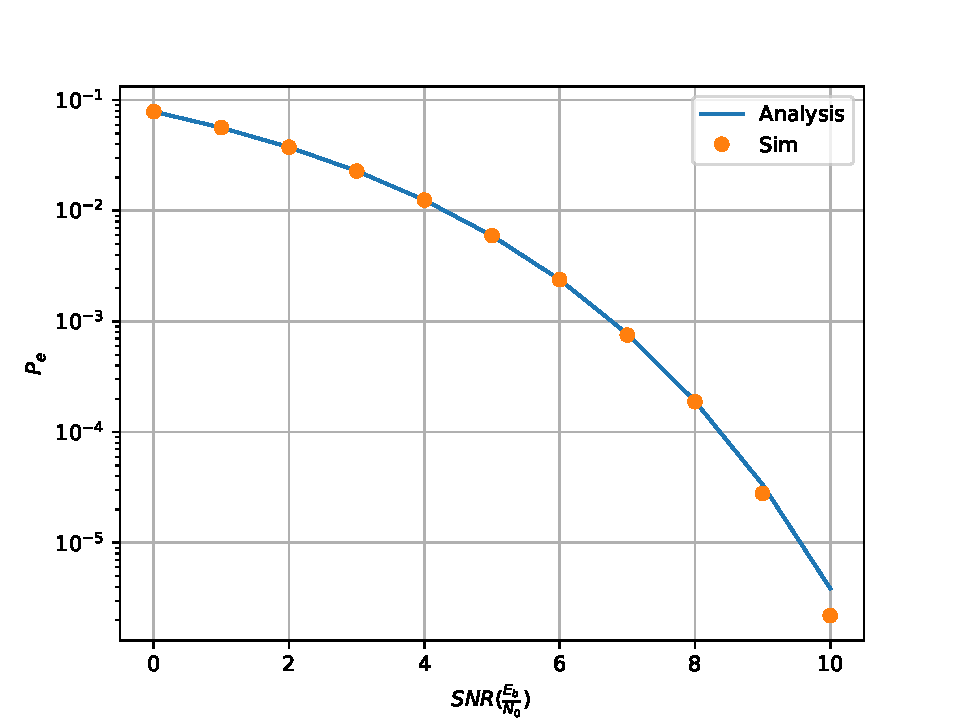
\includegraphics[width=\columnwidth]{./figs/chapter6/bpsk_ber.pdf}
\caption{}
\label{fig:bpsk_ber}
\end{figure}

\item
\label{prob:craigs_formula_proof}
Show that
\begin{equation}
Q(x) = \frac{1}{\pi}\int^{\frac{\pi}{2}}_{0}e^{-\frac{x^2}{2\sin^2 \theta}}\,d\theta
\end{equation}\\
\solution Consider the bivariate gaussian distribution of $X,Y \sim \gauss{0}{1}$,
\begin{equation}
	p_{X,Y}(x,y) = \frac{1}{2\pi}\exp\left(-\frac{x^2+y^2}{2}\right)
	\label{eq:bivariate_std_gaussian_pdf}
\end{equation}
Using $p_{X,Y}(x,y)$, the Q-function can be expressed as,
\begin{align}
	Q(z) &= \int_{z}^{\infty}\int_{-\infty}^{\infty} p_{X,Y}(x,y) \,dx\,dy \\
	\label{eq:qfunc_biv_integ}
	&= \frac{1}{2\pi}\int_{z}^{\infty}\int_{-\infty}^{\infty} \exp\left(-\frac{x^2+y^2}{2}\right) \,dx\,dy
\end{align}
Transforming the integral in \eqref{eq:qfunc_biv_integ} to polar coordinates $(r,\theta)$ for $z > 0$,
\begin{align*}
	Q(z) &= \frac{1}{2\pi}\int_{-\frac{\pi}{2}}^{\frac{\pi}{2}}\int_{\frac{z}{\sin\theta}}^{\infty} \exp\left(-\frac{r^2}{2}\right)r \,dr\,d\theta\\
	&= \frac{1}{2\pi}\int_{-\frac{\pi}{2}}^{\frac{\pi}{2}} \exp\left(-\frac{z^2}{2\sin^2\theta}\right) \,d\theta\\
	&= \frac{1}{\pi}\int_{0}^{\frac{\pi}{2}} \exp\left(-\frac{z^2}{2\sin^2\theta}\right) \,d\theta \text{ , for $z > 0$}
\end{align*}
\end{enumerate}
\section{Coherent BFSK}
\begin{enumerate}
\item
The signal constellation for binary frequency shift keying (BFSK) is given in \figref{fig:bfsk_const}.
Obtain the equations for the received symbols.

\begin{figure}[H]
\centering
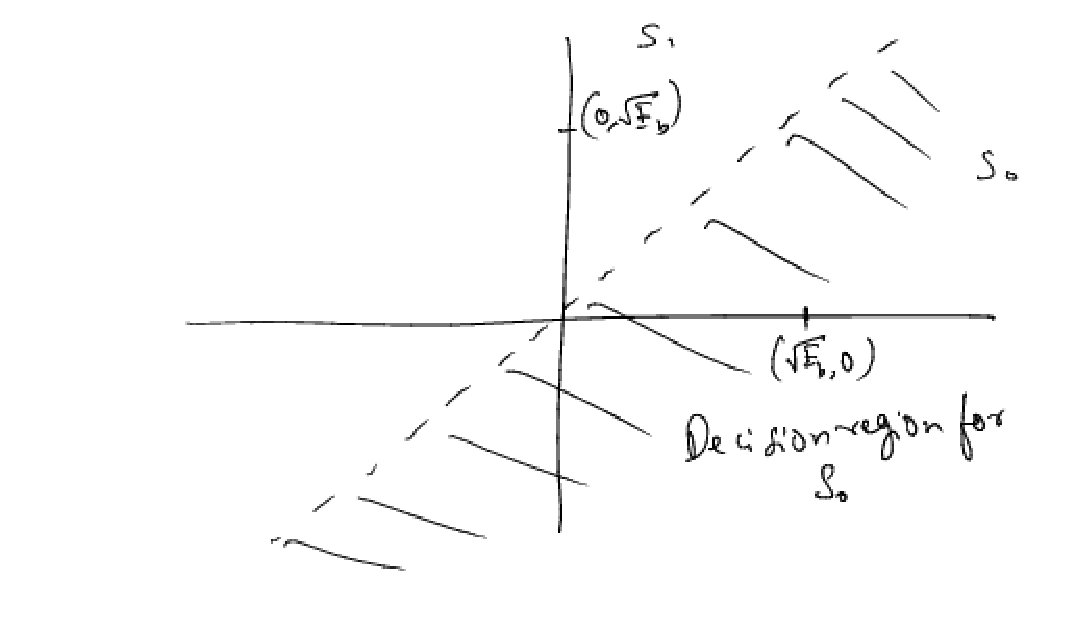
\includegraphics[width=\columnwidth]{./figs/chapter6/bfsk_const.pdf}
\caption{}
\label{fig:bfsk_const}
\end{figure}
\solution
The received symbols are given by
\begin{align}
\mathbf{y}|s_0 = 
\myvec{
\sqrt{E_b} \\
0
}
+
\myvec{
 n_{1}\\
n_{2}
},
\end{align}
and 
\begin{align}
\mathbf{y}|s_1 = 
\myvec{
0\\
\sqrt{E_b} 
}
+
\myvec{
n_{1}\\
 n_{2}
},
\end{align}
where $n_1,n_2 \sim \gauss{0}{\frac{N_0}{2}}$. and
$
\mathbf{y} = 
\myvec{
y_{1}\\
 y_{2}
}
$.
\item
Obtain a decision rule for BFSK from \figref{fig:bfsk_const}.

\solution The decision rule is
\begin{equation}
y_1 \dec{s_0}{s_1} y_2
\end{equation}
\item
Repeat the previous exercise using the MAP criterion.\\
\solution Let $\mbf{y} = \myvec{y_1&y_2&...&y_n}^T$ be the received signal. For an AWGN channel, given that symbol $\mbf{s_k}$ was sent, %
every component $y_i$ is normally distributed i.e. 
\begin{equation}
y_i|\mbf{s_k} \sim \gauss{s_{ki}}{\frac{N_0}{2}}\text{   ,} i=1,2,...,n 
\end{equation}
where $s_{ki}$ is the i$^{th}$ component of symbol $\mbf{s_k}$. Since all components of $\mbf{y}$ are independent, the joint PDF of $\mbf{y}$ given %
$\mbf{s_k}$ was sent is,
\begin{align}
	p_{\mbf{y}}(\mbf{y}|\mbf{s_k}) &= \prod\limits_{i=1}^{n} p_{y_i}(y_i|\mbf{s_k})&\\
	&= \left(\frac{2}{N_0\sqrt{2\pi}}\right)^n \exp\left(-\frac{2}{N_0^2}\sum\limits_{i=1}^{n} (y_i-s_{ki})^2\right)\\
	\label{eq:joint_pdf_fdistance}
	&= \left(\frac{2}{N_0\sqrt{2\pi}}\right)^n \exp\left(-\frac{2}{N_0^2}\norm{\vec{y}-\vec{s_k}}^2\right)
\end{align}
Ignoring the constants in \eqref{eq:joint_pdf_fdistance},
\begin{equation}
	p_{\mbf{y}}(\mbf{y}|\mbf{s_k}) \propto \exp\left(-\norm{\vec{y}-\vec{s_k}}^2\right)
\end{equation}
According to the MAP rule in \eqref{eq:mle_rule}, the optimal criterion to estimate $\vec{s}$ is to choose $\vec{\hat{s}}=\vec{s_k}$ whose
distance from $\vec{y}$ is minimum.
\begin{align}
	\label{eq:AWGN_est_rule}
	\text{Set } \hat{s} &= s_k \text{ if}&\\ \nonumber
	\norm{\vec{y}-\vec{s_i}}^2 & \text{ is minimum for } i = k
\end{align}
For the case of coherent BFSK, the locus for point equidistant from $\vec{s_0}$ and $\vec{s_1}$ is the line $y_1-y_2=0$. So, the optimum
decision is found as 
\begin{equation}
y_1 \dec{s_0}{s_1} y_2
\end{equation}

\item
Derive and plot the probability of error.  Verify through simulation.\\
\solution 
\begin{align}
	P_e &= \pr{y_1<y_2|s_0}\\
	&= \pr{\sqrt{E_b}+n_1<n_2}\\
	&= \pr{n_2-n_1 > \sqrt{E_b}}\\ \nonumber
	&= \pr{z > \sqrt{E_b}}, \text{where $z \sim \gauss{0}{N_0}$}\\
	&= \qfunc{\sqrt{\frac{E_b}{N_0}}}
\end{align}
The following code,
\begin{lstlisting}
codes/chapter6/bfsk_coherent_ber.py
\end{lstlisting}
yields \figref{fig:bfsk_coherent_ber}
\begin{figure}[H]
\centering
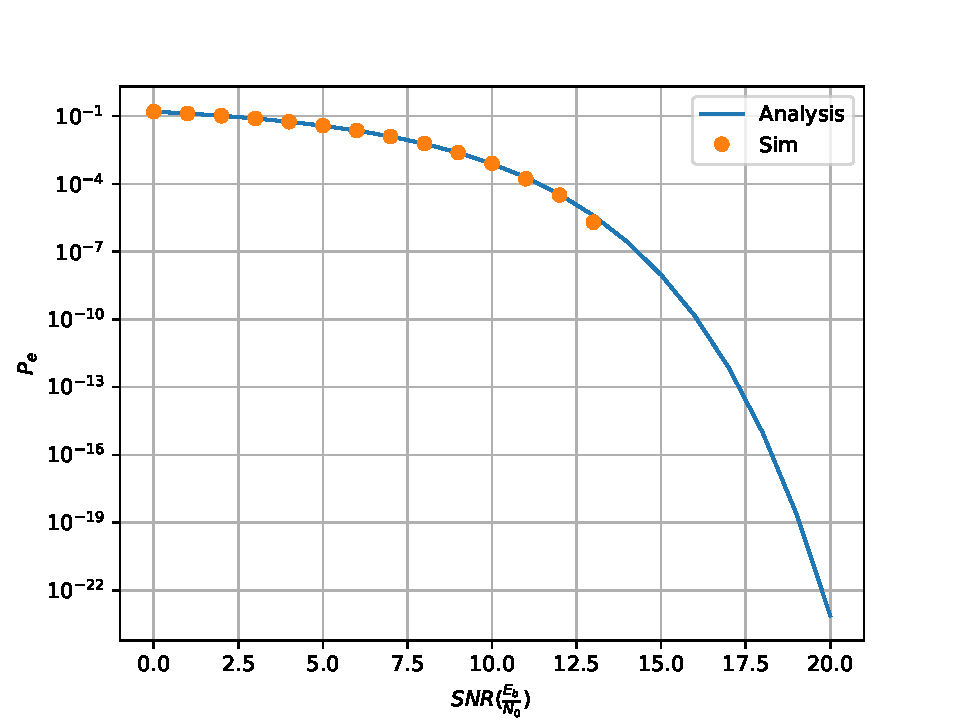
\includegraphics[width=\columnwidth]{./figs/chapter6/bfsk_coherent_ber.pdf}
\caption{$P_e$ versus SNR for coherent BFSK}
\label{fig:bfsk_coherent_ber}
\end{figure}
\end{enumerate}

%
\section{QPSK}
\begin{enumerate}
\item
Let
\begin{equation}
\mathbf{r} = \mathbf{s}+ \mathbf{n}
\end{equation}
where $\mathbf{s} \in \cbrak{s_0,s_1,s_2, s_3}$ and
\begin{align}
\mathbf{s}_0 &= 
\myvec{
\sqrt{E_b}\\
0
},
\mathbf{s}_1 = 
\myvec{
0\\
\sqrt{E_b}
},
\\
\mathbf{s}_2 &= 
\myvec{
-\sqrt{E_b}\\
0
},
\mathbf{s}_3 = 
\myvec{
0\\
-\sqrt{E_b}
},
\\
E\sbrak{\mathbf{n}} &= \mathbf{0}, E\sbrak{\mathbf{n}\mathbf{n}^T} = \sigma^2 \mathbf{I}
\end{align}
%
\begin{enumerate}[label=(\alph{enumii})]
\item Show that the MAP decision for detecting $\mathbf{s}_0$ results in
\begin{equation}
\abs{r}_2 < r_1
\end{equation}\\
\solution For choosing $\vec{\hat{s}} = \vec{s_0}$, the below inequalities have to be satisfied (from \eqref{eq:AWGN_est_rule}).
\begin{align}
	\label{eq:qpsk_map_ineq1}
	\norm{\vec{r}-\vec{s_0}}^2 &< \norm{\vec{r}-\vec{s_1}}^2	\\
	\label{eq:qpsk_map_ineq2}
	\norm{\vec{r}-\vec{s_0}}^2 &< \norm{\vec{r}-\vec{s_2}}^2	\\
	\label{eq:qpsk_map_ineq3}
	\norm{\vec{r}-\vec{s_0}}^2 &< \norm{\vec{r}-\vec{s_3}}^2	
\end{align} 
Simplifying \eqref{eq:qpsk_map_ineq1},
\begin{align*}
	(\vec{r}-\vec{s_0})^{\top}(\vec{r}-\vec{s_0}) &< (\vec{r}-\vec{s_1})^{\top}(\vec{r}-\vec{s_1})\\
	\norm{r}^2 -2\vec{s_0}^{\top}\vec{r} + \norm{s_0}^2 &< \norm{r}^2 -2\vec{s_1}^{\top}\vec{r} + \norm{s_1}^2\\
	(\vec{s_1}-\vec{s_0})^{\top}\vec{r} &< 0 \text{\small,   $[\norm{s_0} = \norm{s_1} = \sqrt{E_b}$]}\\
	\myvec{-\sqrt{E_b}\\\sqrt{E_b}}^{\top}\vec{r} &< 0\\
	\myvec{-1\\1}^{\top}\vec{r} &< 0\\
	r_2 &< r_1
\end{align*}
Similarly, simplifying \eqref{eq:qpsk_map_ineq2} and \eqref{eq:qpsk_map_ineq3} we obtain
\begin{align*}
	r_2 &< r_1	\\
	-r_2 &< r_1 \\
	0 &< r_1	\\
	\implies \abs{r}_2 &< r_1
\end{align*} 

\item Express $\pr{\hat{\mathbf{s}} = \mathbf{s}_0|\mathbf{s} = \mathbf{s}_0}$ in terms of $r_1, r_2$.
Let $X=n_2-n_1, Y = -n_2-n_1$, where $\mathbf{n}=\brak{n_1,n_2}$.
Their correlation coefficient is defined as
%
\begin{align}
\rho = \frac{E\sbrak{\brak{X-\mu_x}\brak{Y-\mu_y}}}{\sigma_x\sigma_y}
\end{align}
%
$X$ and $Y$ are said to be uncorrelated if $\rho = 0$\\
\solution
\begin{flalign}
	\nonumber
	\pr{\hat{\mathbf{s}} = \mathbf{s}_0|\mathbf{s} = \mathbf{s}_0} &= \pr{\abs{r}_2 < r_1 | \mathbf{s} = \mathbf{s}_0}&\\
	\label{eq:qpsk_prob_error_r12}
	&= \pr{r_2 < r_1, -r_2 < r_1| \mathbf{s} = \mathbf{s}_0}
\end{flalign}
\
\item Show that if $X$ and $Y$ are uncorrelated 
Verify this numerically.\\
\solution Since $n_1$ and $n_2$ are independent,
\begin{align}
	p_{n_1,n_2}\brak{n_1,n_2} &= p_{n_1}\brak{n_1}p_{n_2}\brak{n_2}\\
	&= \frac{1}{2\pi\sigma} e^{-\frac{n_1^2+n_2^2}{2\sigma^2}}
\end{align}
Finding $\mu_x = E\sbrak{X}$,
\begin{align*}
	E\sbrak{X} &= E\sbrak{n_2-n_1}\\
	&= \int_{-\infty}^{\infty} \int_{-\infty}^{\infty} \brak{n_2-n_1}p_{n_1,n_2}\brak{n_1,n_2}  \,dn_1  \,dn_2\\
	&= \frac{1}{2\pi\sigma} \int_{-\infty}^{\infty} \int_{-\infty}^{\infty} \brak{n_2-n_1}e^{-\frac{n_1^2+n_2^2}{2\sigma^2}} \,dn_1  \,dn_2
\end{align*}
	
\begin{multline*}
	= \frac{1}{\sqrt{2\pi \sigma}}\left[ \int_{-\infty}^{\infty} e^{-\frac{n_2^2}{2\sigma^2}} \,dn_2 \right.\\
	\left. \frac{1}{\sqrt{2\pi \sigma}}\int_{-\infty}^{\infty} \brak{n_2-n_1} e^{-\frac{n_1^2}{2\sigma^2}} \,dn_1\right]
\end{multline*}
\begin{align*}
	&= \frac{1}{\sqrt{2\pi \sigma}} \int_{-\infty}^{\infty} n_2 e^{-\frac{n_2^2}{2\sigma^2}} \,dn_2\\
	&= 0
\end{align*} 
Similarly $\mu_y = 0$. Substituting $X, Y, \mu_x$ and $\mu_y$ in $\rho$,
\begin{align*}
	\rho &= \frac{E\sbrak{\brak{n_2-n_1}\brak{-n_2-n_1}}}{\sigma_X\sigma_Y}\\
	&= \frac{1}{\sigma_X \sigma_Y} \int_{-\infty}^{\infty} \int_{-\infty}^{\infty} \brak{n_1^2-n_2^2}p_{n_1,n_2}\brak{n_1,n_2}  \,dn_1  \,dn_2\\
	&= \frac{1}{\sigma_X \sigma_Y} \frac{1}{2\pi\sigma} \int_{-\infty}^{\infty} \int_{-\infty}^{\infty} \brak{n_1^2-n_2^2} e^{-\frac{n_1^2+n_2^2}{2\sigma^2}} \,dn_1  \,dn_2
\end{align*}
\begin{multline*}
	= \frac{1}{\sigma_X \sigma_Y} \frac{1}{\sqrt{2\pi \sigma}}\left[ \int_{-\infty}^{\infty} e^{-\frac{n_2^2}{2\sigma^2}} \,dn_2\right. \\
	\left. \frac{1}{\sqrt{2\pi \sigma}}\int_{-\infty}^{\infty} \brak{n_1^2-n_2^2} e^{-\frac{n_1^2}{2\sigma^2}} \,dn_1\right]
\end{multline*}
\begin{align*}
	&= \frac{1}{\sigma_x \sigma_y} \frac{1}{\sqrt{2\pi \sigma}} \int_{-\infty}^{\infty} \brak{\sigma^2-n_2^2} e^{-\frac{n_2^2}{2\sigma^2}} \,dn_2\\
	&= \frac{1}{\sigma_X \sigma_Y} \brak{\sigma^2-\sigma^2}\\
	&= 0
\end{align*}
The code below can be used to verify numerically that $\rho = 0$,
\begin{lstlisting}
codes/chapter6/zero_corr_verify.py
\end{lstlisting}
The output of the code is,
\begin{lstlisting}
Correlation coefficient is: 0.0002998	
\end{lstlisting}
The scatter plot in \figref{fig:zero_corr_scatter} visually shows that there is no significant correlation between $X$ and $Y$.
\begin{figure}[H]
\centering
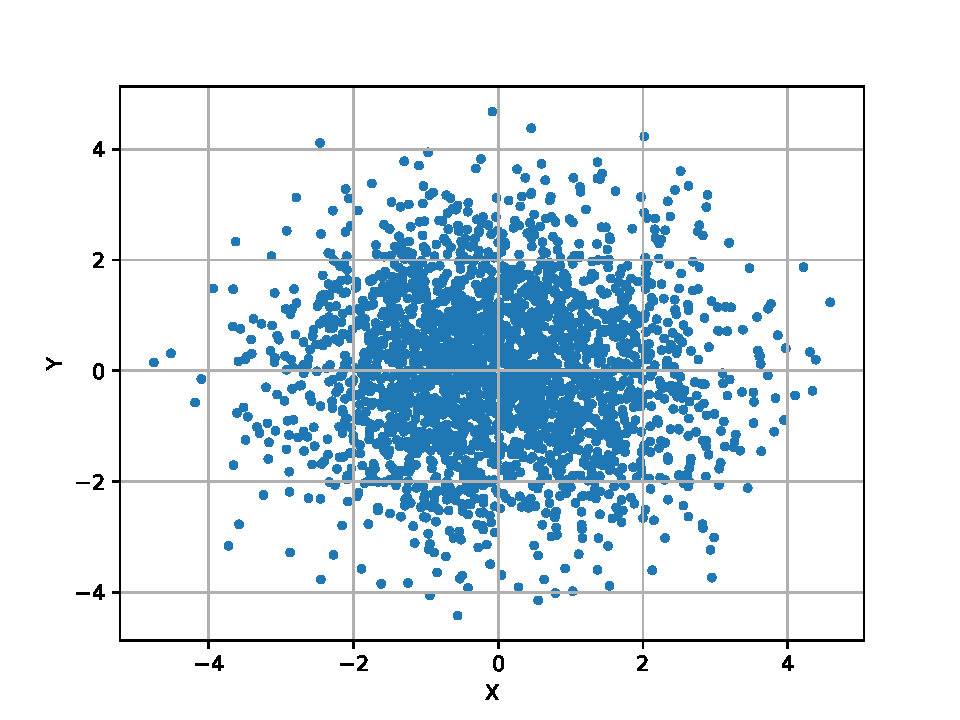
\includegraphics[width=\columnwidth]{./figs/chapter6/zero_corr_verify.pdf}
\caption{Scatter plot of $X$ and $Y$}
\label{fig:zero_corr_scatter}
\end{figure}

\item Show that $X$ and $Y$ are independent, i.e. $p_{XY}(x,y) = p_{X}(x)p_{Y}(y)$.\\
\solution Since $X$ and $Y$ are linear combinations of Gaussian variables, $X$ and $Y$ are normally distributed. The joint PDF of two Gaussian %
variables is given by
\begin{multline}
	\label{eq:biv_gauss_gen}
	p_{X,Y}\brak{x,y} = \frac{1}{2\pi\sigma_X\sigma_Y\sqrt{1-\rho^2}}\\
	\exp\left\{-\frac{1}{2\brak{1-\rho^2}}\left[\brak{\frac{x-\mu_X}{\sigma_X}}^2+\brak{\frac{y-\mu_Y}{\sigma_Y}}^2\right.\right.\\
	\left.\left.-2\rho\frac{\brak{x-\mu_X}\brak{Y-\mu_Y}}{\sigma_X\sigma_Y}\right]\right\}
\end{multline}
Substituting $\rho = 0$,  
\begin{align}
	p_{X,Y}\brak{x,y} &= \frac{1}{2\pi\sigma_X\sigma_Y}\exp\cbrak{-\frac{\brak{x-\mu_X}^2}{2\sigma_X^2}-\frac{\brak{y-\mu_Y}^2}{2\sigma_Y^2}}\\
	&= \frac{1}{\sigma_X\sqrt{2\pi}}e^{-\frac{\brak{x-\mu_x}^2}{2\sigma_X^2}} \frac{1}{\sigma_Y\sqrt{2\pi}}e^{-\frac{\brak{y-\mu_y}^2}{2\sigma_Y^2}}\\
	&= p_X\brak{x} p_Y\brak{y}
\end{align}
\item Show that $X,Y \sim \mathcal{N}\brak{0,2\sigma^2}$.\\
\solution $X = n_2-n_1$ where $n_2, -n_1 \sim \gauss{0}{\sigma^2}$. The PDF of X is given by,
\begin{align}
	\nonumber
	p_X(x) &= p_{n_2}(n_2) \ast p_{-n_1}(n_1)\\\nonumber
	&= \frac{1}{2\pi\sigma^2}\int_{-\infty}^{\infty} e^{-\frac{t^2}{2\sigma^2}}e^{-\frac{(x-t)^2}{2\sigma^2}}  \,dt\\\nonumber
	&= \frac{1}{2\pi\sigma^2}\int_{-\infty}^{\infty} e^{-\frac{(x-t)^2+t^2}{2\sigma^2}}  \,dt\\\nonumber
	&= \frac{1}{2\pi\sigma^2}\int_{-\infty}^{\infty} e^{-\frac{(2t-x)^2+x^2}{2(\sqrt{2}\sigma)^2}}  \,dt\\\nonumber
	&= \frac{1}{2\pi\sigma^2}e^{-\frac{x^2}{2(\sqrt{2}\sigma)^2}}\int_{-\infty}^{\infty} e^{-\frac{(2t-x)^2}{2(\sqrt{2}\sigma)^2}}  \,dt\\\nonumber
	&= \frac{e^{-\frac{x^2}{2(\sqrt{2}\sigma)^2}}}{\sqrt{2\pi}\sqrt{2}\sigma} \frac{1}{\sqrt{2\pi}\sqrt{2}\sigma}\int_{-\infty}^{\infty} e^{-\frac{k^2}{2(\sqrt{2}\sigma)^2}}  \,dk\\
	\label{eq:std_gauss_diff_pdf}
	&= \frac{e^{-\frac{x^2}{2(\sqrt{2}\sigma)^2}}}{\sqrt{2\pi}\sqrt{2}\sigma}
\end{align}
From \eqref{eq:std_gauss_diff_pdf}, $X \sim \gauss{0}{2\sigma^2}$. Since $n_2$ and $-n_2$ are identically distributed (due to zero mean),
\begin{align*}
	p_Y(y) &= p_{-n_2}(n_2) \ast p_{-n_1}(n_1)\\
	&= p_{n_2}(n_2) \ast p_{-n_1}(n_1)\\
	&= p_X(x)
\end{align*}
So, $X,Y \sim \gauss{0}{2\sigma^2}$.
\item Show that $\pr{\hat{\mathbf{s}} = \mathbf{s}_0|\mathbf{s} = \mathbf{s}_0} =\pr{ X < A,  Y < A}$.\\
\solution From \eqref{eq:qpsk_prob_error_r12},
\begin{flalign*}
	\pr{\hat{\mathbf{s}} = \mathbf{s}_0| \mathbf{s} = \mathbf{s}_0} = \pr{r_2 < r_1, -r_2 < r_1 | \mathbf{s} = \mathbf{s}_0}&\\
	= \pr{n_2<n_1+\sqrt{E_b}, -n_2<n_1+\sqrt{E_b}}&\\
	= \pr{n_2-n_1<\sqrt{E_b}, -n_2-n_1<\sqrt{E_b}}&\\
	= \pr{X<\sqrt{E_b}, Y<\sqrt{E_b}}&\\
	= \pr{X<A, Y<A}
\end{flalign*}
\item Find $\pr{ X < A,  Y < A}$.\\
\solution Since $X$ and $Y$ are independant, 
\begin{flalign*}
	\pr{ X < A,  Y < A} = \pr{X<A}\pr{Y<A}
\end{flalign*}%
\begin{flalign*}
	&= F_X(A)F_Y(A)&\\
	&= \left(1-\qfunc{\frac{A}{\sqrt{2}\sigma}}\right)\left(1-\qfunc{\frac{A}{\sqrt{2}\sigma}}\right)&\\
	&= \left(1-\qfunc{\frac{A}{\sqrt{2}\sigma}}\right)^2&\\
	&= \left(1-\qfunc{\sqrt{\frac{E_b}{N_0}}}\right)^2 &\\
	& \text{since } A=\sqrt{E_b}, \sigma=\sqrt{\frac{N_0}{2}}&\\
	&= 1-2\qfunc{\sqrt{\frac{E_b}{N_0}}}+\qfunc{\sqrt{\frac{E_b}{N_0}}}^2&\\
	&\approx 1-2\qfunc{\sqrt{\frac{E_b}{N_0}}}&\\
	&= 1-\operatorname{erfc}\left(\sqrt{\frac{E_b}{2N_0}}\right)
\end{flalign*}
\item Verify the above through simulation.\\
\solution 
The following code,
\begin{lstlisting}
codes/chapter6/qfsk_ber.py
\end{lstlisting}
yields \figref{fig:qpsk_ber}. $P_e = 1-\pr{X<A,Y<A}$ plotted for SNR values from 0 to 10.
\begin{figure}[H]
\centering
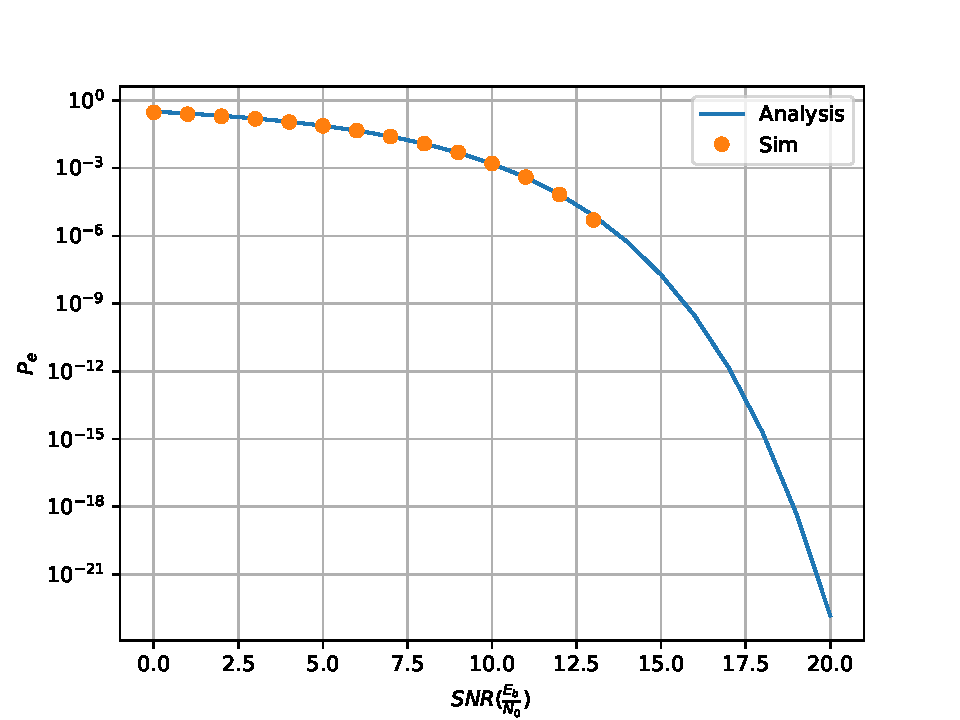
\includegraphics[width=\columnwidth]{./figs/chapter6/qpsk_ber.pdf}
\caption{}
\label{fig:qpsk_ber}
\end{figure}
\end{enumerate}
\end{enumerate}

\section{$M$-PSK}
\begin{enumerate}

\item
Consider a system where 
$\mathbf{s}_i=
\myvec{
\cos\brak{\frac{2\pi i}{M}}\\
\cos\brak{\frac{2\pi i}{M}}
}, i = 0, 1 , \dots M-1
$
.
Let
%
\begin{align}
\mathbf{r}|s_0 = 
\myvec{
r_1\\
r_2
}
=
\myvec{
\sqrt{E_s}+n_1\\
n_2
}
\end{align}
where $n_1,n_2 \sim \mathcal{N}\brak{0,\frac{N_0}{2}}$.

\begin{enumerate}[label=(\alph{enumii})]
\item Substituting 
\begin{align}
r_1=R\cos \theta \\
r_2=R\sin \theta
\end{align}
show that the joint pdf of $R,\theta$ is
%
\begin{equation}
p\brak{R,\theta}=\frac{R}{\pi N_0}\exp\brak{-\frac{R^2-2R\sqrt{E_s}\cos \theta + E_s}{N_0}}
\end{equation}
%
\item Show that 
%
\begin{align}
\lim_{\alpha \rightarrow \infty}\int_{0}^{\infty}\brak{V-\alpha }e^{-\brak{V-\alpha}^2 }\,dV
&= 0
\\
\lim_{\alpha \rightarrow \infty}\int_{0}^{\infty} e^{-\brak{V-\alpha}^2 }\,dV
&=  \sqrt{\pi}
\end{align}
%
\item 
Using the above, evaluate
%
\begin{align}
\int_{0}^{\infty}V\exp\cbrak{-\brak{V^2 - 2V \sqrt{\gamma}\cos \theta +\gamma}}\,dV
\end{align}
%
for large values of $\gamma$.
\item
Find a compact expression for 
%
\begin{align}
I = 1 - \sqrt{\frac{\gamma}{\pi}}\int_{-\frac{\pi}{M}}^{\frac{\pi}{M}}e^{- \gamma\sin^2\theta }\cos \theta\, d\theta
\end{align}
\item Find $P_{e|\mathbf{s}_0}$.
\end{enumerate}
\end{enumerate}
\section{Noncoherent BFSK}
\begin{enumerate}
\item
Show that
%
\begin{align}
I_{0}(x) &= \frac{1}{2\pi}\int_{0}^{2\pi}e^{x\cos\theta}\,d\theta \\
I_{0}(x) &= \frac{1}{2\pi}\int_{0}^{2\pi}e^{x\cos\brak{\theta-\phi}}\,d\theta \\
\frac{1}{2\pi}\int_{0}^{2\pi}e^{m_1\cos\theta + m_2\sin\theta}\,d\theta &= I_0\brak{\sqrt{m_1^2+m_2^2}} 
\end{align}
%
where the modified Bessel function of order $n$ (integer) is defined as 
%
\begin{align}
I_{n}(x) = \frac{1}{\pi}\int_{0}^{\pi}e^{x\cos\theta}\cos n\theta\,d\theta
\end{align}
\item
Let
%
\begin{align}
\mathbf{r}|0= \sqrt{E_b}
\myvec{
\cos \phi_0\\
\sin \phi_0 \\
0\\
0
}
+\mathbf{n}_0,
\mathbf{r}|1= \sqrt{E_b}
\myvec{
0\\
0 \\
\cos \phi_1\\
\sin \phi_1 
}
+\mathbf{n}_1
\end{align}
%
where $\mathbf{n}_0,\mathbf{n}_1\sim \mathcal{N}\brak{\mathbf{0}, \frac{N_0}{2}\mathbf{I}}$.
%
\begin{enumerate}[label=(\alph{enumii})]
\item Taking $\mathbf{r} = \brak{r_1,r_2,r_3,r_4}^{T},$, find the pdf $p\brak{\mathbf{r}|0,\phi_0}$ in
terms of $r_1,r_2,r_3,r_4,\phi,E_b$ and $N_0$. Assume that all noise variables are independent.
%
\item 
If $\phi_0$ is uniformly distributed between 0 and $2\pi$, find $p\brak{\mathbf{r}|0}$.  Note that this expression will no longer contain $\phi_0$.
%
\item
Show that the ML detection criterion for this scheme is
%
\begin{align}
I_0\brak{k\sqrt{r_1^2+r_2^2}}\dec{0}{1}I_0\brak{k\sqrt{r_3^2+r_4^2}}
\end{align}
%
where $k$ is a constant.
%
\item 
The above criterion reduces to something simpler.  Can you guess what it is?  Justify your answer.
%
\item 
Show that 
%
\begin{align}
P_{e|0}=\pr{r_1^2+r_2^2 < r_3^2+r_4^2 | 0}
\end{align}
%
\item 
Show that the pdf of $Y=r_3^2+r_4^2$ id
%
\begin{align}
p_{Y}(y) = \frac{1}{N_0}e^{-\frac{y}{N_0}}, y > 0
\end{align}
%
\item 
Find 
%
\begin{align}
g\brak{r_1,r_2} = \pr{r_1^2+r_2^2<Y|0,r_1,r_2}.
\end{align}
\item 
Show that $E\sbrak{e^{-\frac{X^2}{2\sigma^2}}}=\frac{1}{\sqrt{2}}e^{-\frac{\mu^2}{4\sigma^2}}$ for $X \sim 
\mathcal{N}\brak{\mu,\sigma^2}$.
%
\item 
Now show that
%
\begin{align}
E\sbrak{g\brak{r_1,r_2}}=\frac{1}{2}e^{-\frac{E_b}{2N_0}}.
\end{align}
%
\end{enumerate}
\item
 Let $U,V\sim\mathcal{N}\brak{0,\frac{k}{2}}$ be i.i.d.  Assuming that
%
\begin{align}
U = \sqrt{R} \cos \Theta \\
V = \sqrt{R} \sin \Theta
\end{align}
\begin{enumerate}[label=(\alph{enumii})]
\item 
Compute the jacobian for $U,V$ with respect to $X$ and $\Theta$ defined by
%
\begin{align}
J = \det\brak{
\begin{matrix}
\frac{\partial U}{\partial R} & \frac{\partial U}{\partial \Theta} \\
\frac{\partial V}{\partial R} & \frac{\partial V}{\partial \Theta}
\end{matrix}
}
\end{align}
\item 
The joint pdf for $R,\Theta$ is given by,
%
\begin{align}
p_{R,\Theta}\brak{r,\theta} = p_{U,V}\brak{u,v}J\vert_{u = \sqrt{r}\cos\theta,v = \sqrt{r}\sin\theta}
\end{align}
%
Show that
%
\begin{align}
p_{R}(r) = 
\begin{cases}
\frac{1}{k}e^{-\frac{r}{k}} & r > 0, \\
0 & r < 0,
\end{cases}
\end{align}
%
assuming that $\Theta$ is uniformly distributed between 0 to $2\pi$.
\item
Show that the pdf of $Y = R_1-R_2$, where $R_1$ and $R_2$ are i.i.d. and have the same distribution as $R$ is
%
\begin{align}
p_{Y}(y) = \frac{1}{2k}e^{-\frac{\abs{y}}{k}}
\end{align}
%
\item 
 Find the pdf of 
%
\begin{align}
Z = p + \sqrt{p}\sbrak{U \cos \phi + V \sin \phi}
\end{align}
%
where $\phi$ is a constant.
\item 
Find $\pr{Y > Z}$.
\item 
If $U\sim\mathcal{N}\brak{m_1,\frac{k}{2}},V\sim\mathcal{N}\brak{m_2,\frac{k}{2}}$, where $m_1,m_2, k$ are constants, show that the pdf of 
%
\begin{align}
R = \sqrt{U^2+V^2}
\end{align}
%
is
%
\begin{align}
p_{R}\brak{r} = \frac{e^{-\frac{r +m}{k}}}{ k}I_{0}\brak{\frac{2\sqrt{mr}}{k}},\quad m = \sqrt{m_1^2+m_2^2}
\end{align}
%
\item
Show that
\begin{align}
I_0(x) = \sum_{n=0}^{\infty}\frac{x^{2n}}{4^n\brak{n!}^2}
\end{align}
\item 
If
%
\begin{align}
p_{Z}(z) &= 
\begin{cases}
\frac{1}{k} e^{-\frac{z}{k}} & z \geq 0 \\
0 & z < 0
\end{cases}
\end{align}
%
find $\pr{R < Z}$.
\end{enumerate}
\end{enumerate}
\section{Craig's Formula and MGF}
\begin{enumerate}
\item
The Moment Generating Function (MGF) of $X$ is defined as
%
\begin{align}
M_{X}(s) = E\sbrak{e^{s X}}
\end{align}
%
where $X$ is a random variable and $E\sbrak{\cdot}$ is the expectation.  
%
%
\begin{enumerate}[label=(\alph{enumii})]
\item Let $Y \sim \gauss{0}{1}$.  Define
%
\begin{align}
Q(x) = \pr{Y > x}, x > 0
\end{align}
%
Show that
\begin{equation}
Q(x) = \frac{1}{\pi}\int^{\frac{\pi}{2}}_{0}e^{-\frac{x^2}{2\sin^2 \theta}}\,d\theta
\end{equation}
\item 
Let $h\sim\mathcal{CN}\brak{0,\frac{\Omega}{2}},n\sim\mathcal{CN}\brak{0,\frac{N_0}{2}}$.  Find the distribution of $\abs{h}^2$.
\item Let
%
\begin{align}
P_e = \pr{\Re \cbrak{h^*y} < 0}, \text{ where } y = \brak{\sqrt{E_s}h + n},
\end{align}
%
Show that
%
\begin{align}
P_e = \int_{0}^{\infty}\qfunc{\sqrt{2x}}p_{A}(x) \,dx
\end{align}
where $A = \frac{E_s\abs{h}^2}{N_0}$.
\item Show that
%
\begin{align}
P_e 
%&= E\sbrak{\qfunc{\sqrt{2A}}} \\
%&=  \frac{1}{\pi}\int_{0}^{\frac{\pi}{2}}E\sbrak{e^{-\frac{A}{\sin^2\theta}}}\,d\theta \\
&=  \frac{1}{\pi}\int_{0}^{\frac{\pi}{2}}M_{A}\brak{-\frac{1}{\sin^2\theta}}\,d\theta
\label{ch4_pe_mgf}
\end{align}
%
\item compute $M_A(s)$.
%
\item 
Find $P_e$.
\item 
If $\gamma = \frac{\Omega E_s}{N_0}$, show that $P_e < \frac{1}{2\gamma}$. 
\end{enumerate}
\end{enumerate}
%
\end{document}
